% !TEX root = main.tex
\documentclass[a4paper, UKenglish, 11pt]{uiomaster}
\usepackage{lipsum}
\usepackage[subpreambles=true]{standalone}
\usepackage[table,xcdraw]{xcolor}
\usepackage{hyperref}
\usepackage{xcolor}
\usepackage{placeins}

\begin{document}

\chapter{Extending the Feed Forward Neural Network} \label{chap:extended_FFNN}
So far we have seen how a simple FCNN and a compatible convolutional neural network performs in the task of localizing both single and multiple current dipoles. In this chapter, we will delve into how minor adjustments in data design and network architecture can enhance the FCNN's ability to identify various attributes of current dipoles. We will introduce two distinct extensions of the initial inverse problem, which will put the predictive capabilities of the FCNN to the test in handling more complex scenarios.

The first case involves extending the data set by assigning individual magnitudes to each dipole source. This extension presents the network with the task of predicting both location of the source and its corresponding magnitude. The second scenario transitions from predicting the location of a single dipole source to estimating the center and radius of a population of dipoles, while also determining the magnitude of the signal strength of the entire dipole population.

In Section \ref{sec:method}, we will detail the modifications made to the simulated data that is the same for both of the problems, along with the necessary adjustments to the network architecture. Moving on to Sections \ref{sec:result_magnitude} and \ref{sec:result_area}, we will present the distinct data simulation choises for each of the problems, alongside the performance of the network in addressing these more complex challenges.

In Section \ref{sec:method}, we will outline the modifications made to the data and network architecture that have been implemented to address both of the problems. Transitioning to Sections \ref{sec:result_magnitude} and \ref{sec:result_area}, we will delve into the specifics of data simulation tailored to each problem, in addition to evaluating the network's performance when dealing with these more complex problems.

%we methodically introduce distinct modifications to the data and network architecture for each problem, assess the network's performance, and offer insights into its strengths and limitations when addressing these novel challenges.

\section{Method: Adjusting Data Set and Architecture} \label{sec:method}
Before delving into the performance of the FCNN regarding the intricate problems of predicting dipole strengt and radius alongside location, we will address important considerations that apply to both extensions. This encompasses instructing the network on how to handle varying units in its output, selecting an optimal cost function tailored to our specific problems, and establishing criteria for assessing the network's performance in the context of its intended tasks.

% \subsection{Scaling of Target Values}
% In these exteded EEG inverse problems, the target values spans different range and is expressed in different units. When a nerual network is tasked with predicting outputs to which exhibit disparities in their ranges and units, several challenges may arise.
%
% To understand why a neural network may trouble when predicting target values with distinct ranges and units, we remind ours selfs about the pupose of the cost function. Neural networks use cost functions to calculate the differences between predicted output and target values. When a network has multiple outputs, the total cost of the network is the sum of the distinct terms. However, attempting to add together losses from distinct target values with varying units lacks a straightforward and intuitive approach. Combining values with different units into a single loss function can lead to an ambiguous interpretation and hinder the meaningful evaluation of the network's performance. Moreover, the variation in the range of target values poses a potential issue. Variations can result in certain dimensions being imbalanced in their influence on the overall error, potentially overshadowing dimensions with smaller ranges. This asymmetry in the error calculation can lead to a biased optimization process and hinder the network's ability to effectively learn from the data.
%
% This necessitates an essential preprocessing step: the scaling of target data. By instructing the network to output unitless vectors $\textbf{{y}}$ with elements consistent in range between 0 to 1, we help the network overcome these challanges. This instruction can be given to the network by scaling the network's target values $\mathbf{\tilde{y}}_i \in \tilde{\mathcal{Y}}$ for $i \in \{0, N-1\}$, where $N$ is the number of samples. The scaling is done by normalizing each component of the target vector $\tilde{\mathbf{y}_i} = [\tilde{y}_{i,0}, \tilde{y}_{i,1}, ..., \tilde{y}_{i,d-1}]$ separately. Here $d$ denotes the dimension of $\tilde{\mathbf{y}_i}$, i.e. the number of target values contained in each sample. The normalized target value $\tilde{y}_{i,j}'$ of the $i$'th sample for the $j$'th dimension is given as follows:
%
% \begin{equation}
% \tilde{y}_{i,j}' = \frac{\tilde{y}_{i,j} - \text{min}(\{\tilde{\mathbf{y}}\}_j)}{\text{max}(\{\tilde{\mathbf{y}}\}_j) - \text{min}(\{\tilde{\mathbf{y}}\}_j)}.
% \label{eq:scale_target}
% \end{equation}
%
% \noindent Here, min($\{\tilde{\mathbf{y}}_j\}$) and max($\{\tilde{\mathbf{y}}_j\}$) denote the minimum and maximum values corresponding to a specific target dimension across all samples. By normalizing the target values in this manner, the neural nework will strive to output predictions with range 0 to 1. Consequencly the cost of the network is calculated by summing the unitless differences between targets where all target values contribute equally to the overall error calculation. Consequently, the neural network can harness its learning capabilities more effectively and hopefully perform better in its tasks.
%
%
\subsection{Scaling of Target Values}
\rednote{Include original ranges one more time?}
In the extended EEG inverse problems, the neural network is tasked with predicting target values that vary significantly in their range and units. To comprehend why this can be problematic, it is essential to revisit the purpose of the cost function. Neural networks employ cost functions to quantify the error between their predicted outputs and the target values. Depending on the cost function utilized, this error is expressed in units related to the true dimension of the target value. When a neural network has multiple outputs, the overall cost is determined by the sum of distinct errors corresponding to each output. However, adding together error terms with distinct units is a non-intuitive task. Letting the network do so, may lead to an ambiguous interpretation of the cost and hinder meaningful evaluation of the network's performance. Furthermore, the variation in the range of target values poses an additional challenge. This variation can result in certain domains of the data having an imbalanced influence on the overall error calculation, potentially overshadowing targets with smaller ranges. Such an asymmetry in the error calculation can lead to a biased optimization process and hinder the network's ability to effectively learn from the data.

To address these issues, a preprocessing step is required, which involves scaling of the target data. By instructing the neural network to output unitless vectors $\textbf{{y}}$ with elements constrained within the range of 0 to 1, these challenges can be mitigated. This instruction can be given to the network by scaling the its target values $\mathbf{\tilde{y}}_i \in \tilde{\mathcal{Y}}$ for $i \in \{0, N-1\}$, where $N$ is the number of samples. The scaling is done by normalizing each component of the target vector $\tilde{\mathbf{y}_i} = [\tilde{y}_{i,0}, \tilde{y}_{i,1}, ..., \tilde{y}_{i,d-1}]$ separately. Here, $d$ denotes the dimension of $\tilde{\mathbf{y}_i}$, which corresponds to the number of target values contained in each sample. The normalized target value $\tilde{y}_{i,j}'$ for the $i$'th sample and the $j$'th dimension, is calculated as follows:

\begin{equation}
\tilde{y}_{i,j}' = \frac{\tilde{y}_{i,j} - \text{min}(\{\tilde{\mathbf{y}}\}_j)}{\text{max}(\{\tilde{\mathbf{y}}\}_j) - \text{min}(\{\tilde{\mathbf{y}}\}_j)}.
\label{eq:scale_target}
\end{equation}

In this equation, min($\{\tilde{\mathbf{y}}_j\}$) and max($\{\tilde{\mathbf{y}}_j\}$) represent the minimum and maximum values for a specific target dimension across all samples. By normalizing the target values in this manner, the neural network is guided to produce predictions within the range of 0 to 1. Consequently, the network's cost is computed by summing the unitless errors corresponding to each target prediction, for each dimension, ensuring that all target values contribute equally to the overall error calculation. As a result, the neural network learn more effectively, thereby enhancing its performance in various tasks.



\subsection{Sigmoid as Last Layer Activation Function}
In the context of predicting the postion of a single dipole source, the FFNN did not employ any activation in its final layer. However, given that our output data has been normalized, we find it appropriate to use the \emph{Sigmoid} activation function in the output layer. Sigmoid is a logistic mathematical function that maps its input to a bounded range between 0 and 1, as expressed by the equation:

\begin{equation}
  f(x) = \frac{1}{1 + e^{-x}}.
\label{eq:Sigmoid}
\end{equation}

In Figure \ref{fig:sigmoid} we have provided a visualization of Sigmoid's transformation characteristics. The mapping of input values aligns with our desired output range, with normalized target values for the exteded problems. This choice of activation in the output layer aligns with our desired output range, considering the normalized target values for the extended problem domains. The final layer activation aims to facilitate the training process, constraining the network from generating outputs beyond the intended normalized target range.

\begin{figure}
    \centering
    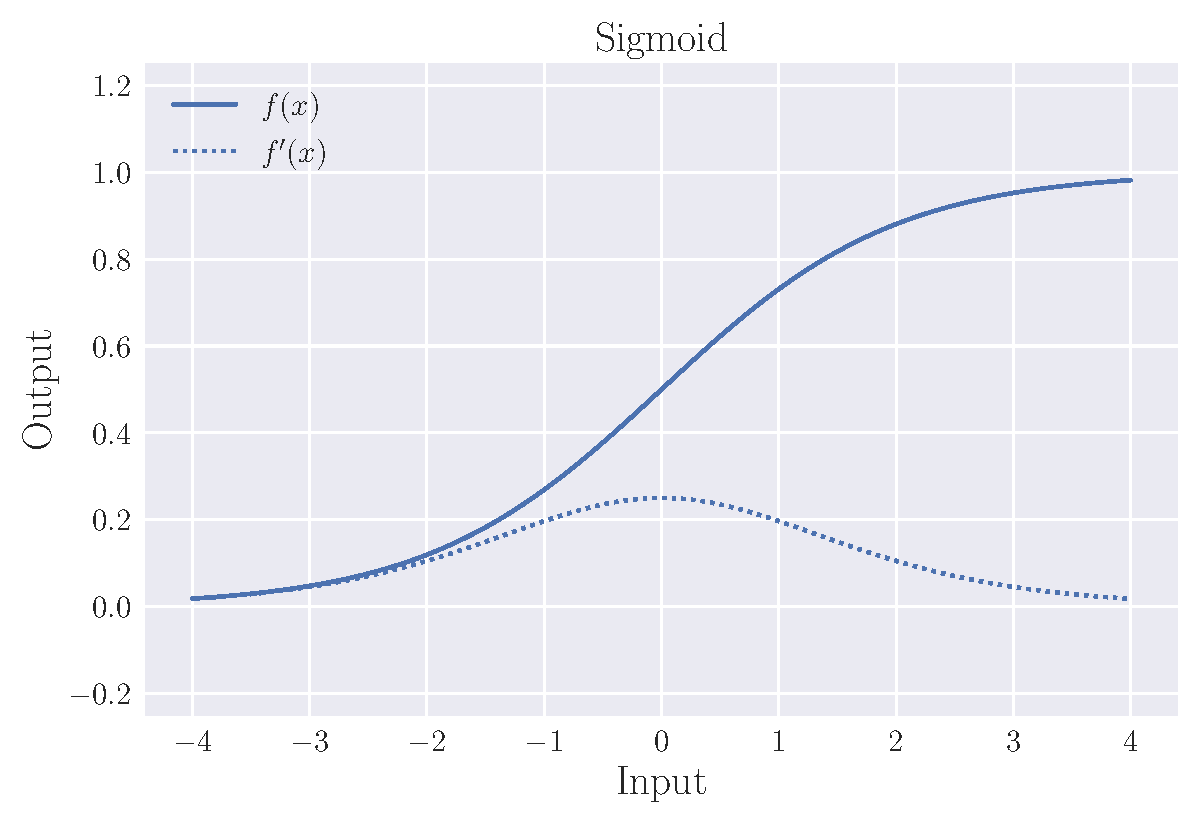
\includegraphics[width=\linewidth]{figures/Sigmoid.pdf}
    \caption{\textbf{Sigmoid activation function}: transforms the input value $x$ into a smooth S-shaped curve, mapping it to a range between 0 and 1.}
    \label{fig:sigmoid}
\end{figure}


% Include data distribution (min/max)
\subsection{Choosing an Optimal Cost Function}
The formulation of a customized cost function tailored to the specific modeling objectives is imperative when confronted with machine learning problems in need of multiple network outputs, each characterized by distinct units and interpretations, such as ours.  We aim to construct a model that can effectively predict not only the spatial coordinates of a current dipole moment but also accurately estimate the dipole's magnitude and the radii associated with a population of multiple current dipoles. To achieve this objective, our ideal cost function comprises several components.

Firstly, it calculates the Euclidean distance between predicted spatial coordinates $x, y, z \in \mathbf{y}$ and correspnding true values $\tilde{x}, \tilde{y}, \tilde{z} \in \mathbf{\tilde{y}}$ for $N$ number of samples:

\begin{equation}
    \text{MED}(\mathbf{y}, \mathbf{\tilde{y}}) = \frac{1}{N}\sum_{i=0}^{N-1}\sqrt{(x_{i} - \tilde{x}_{i})^2 + (y_{i} - \tilde{y}_{i})^2 + (z_{i} - \tilde{z}_{i})^2}.
\label{eq:MED}
\end{equation}

Additionally, the cost function calculates the absolute error between the predicted magnitude ${A} \in \mathbf{y}$ and the true magnitude $\tilde{A} \in \mathbf{\tilde{y}}$:

\begin{equation}
    \text{MAE$_A$}(\mathbf{y}, \mathbf{\tilde{y}}) = \frac{1}{N} \sum_{i=0}^{N-1} | A_{i} - \tilde{A}_{i} |.
\label{eq:MAE_A}
\end{equation}

Similarly, it aims to quantify the absolute error between the predicted radius ${\text{r}} \in \mathbf{y}$ and the true radius $\tilde{\text{r}} \in \mathbf{\tilde{y}}$:

\begin{equation}
    \text{MAE$_r$}(\mathbf{y}, \mathbf{\tilde{y}}) = \frac{1}{N} \sum_{i=0}^{N-1} | r_{i} - \tilde{r}_{i} |
\label{eq:MAE_r}
\end{equation}

\rednote{Remove r=3 (simple dipole) or add r=6 (two dipoles)?}
With an output $\textbf{y} \in \mathcal{Y}(d)$, where $d$ represents the dimension of $\textbf{y}$ and $\mathcal{Y}(d) \subset \mathbb{R}^d$, a collective cost function, tailored for each of the distinct problem scenarios, can be defined as follows:

\begin{equation}
    C(\mathcal{Y}, \mathcal{\tilde{Y}}) =
    \begin{cases}
      \begin{array}{l}
      \text{MED}(x,y,z),
      \end{array} & \text{if } d = 3\\
      \\
      \begin{array}{l}
      \text{MED}(x,y,z) + \text{MAE}(A)
      \end{array} & \text{if } d = 4\\
      \\
      \begin{array}{l}
      \text{MED}(x,y,z) + \text{MAE}(A) + \text{MAE}(r),
      \end{array} & \text{if } d = 5\\
    \end{cases}
    \label{eq:cost_function}
\end{equation}

In the case where $d = 3$, the simplest problem is considered, where the network predicts the coordinates of a single-point current dipole, as explored in Chapter \ref{chap:simple_dipole_FFNN} and Chapter \ref{chap:simple_dipole_CNN}. If $d = 4$, the network predicts the $x$-, $y$-, and $z$-coordinates of a single dipole, in addition to the magnitude $A$ of the signal strength. When $d = 5$, the target vector encompasses all previously mentioned values, along with the radius of a current dipole population.
%Finally, for $| \boldsymbol{\theta} |$ greater than 5, the multiple dipole problem is addressed, where the network predicts the locations for two or more point source dipoles situated at distinct positions within the cortex.

\subsection{Overview on Arcitecture and Hyperparameters}
Figure \ref{fig:NN_dipole_w_amplitude_architecture} presents a visualization of the architecture of the extended FCNN, which is designed to produce $d$ target values depending on the specific problem to solve. The architecture of the FFNN is equal to that employed for both the single dipole problem discussed in Chapter \ref{chap:simple_dipole_FFNN} and the multipole dipole problem examined in Chapter \ref{chap:two_dipole_FFNN}, with 231 input nodes, corresponding to the number of electrode recording measurements for one sample, and retains the same number of hidden nodes and layers.

\begin{figure}[!htb]
    \centering
    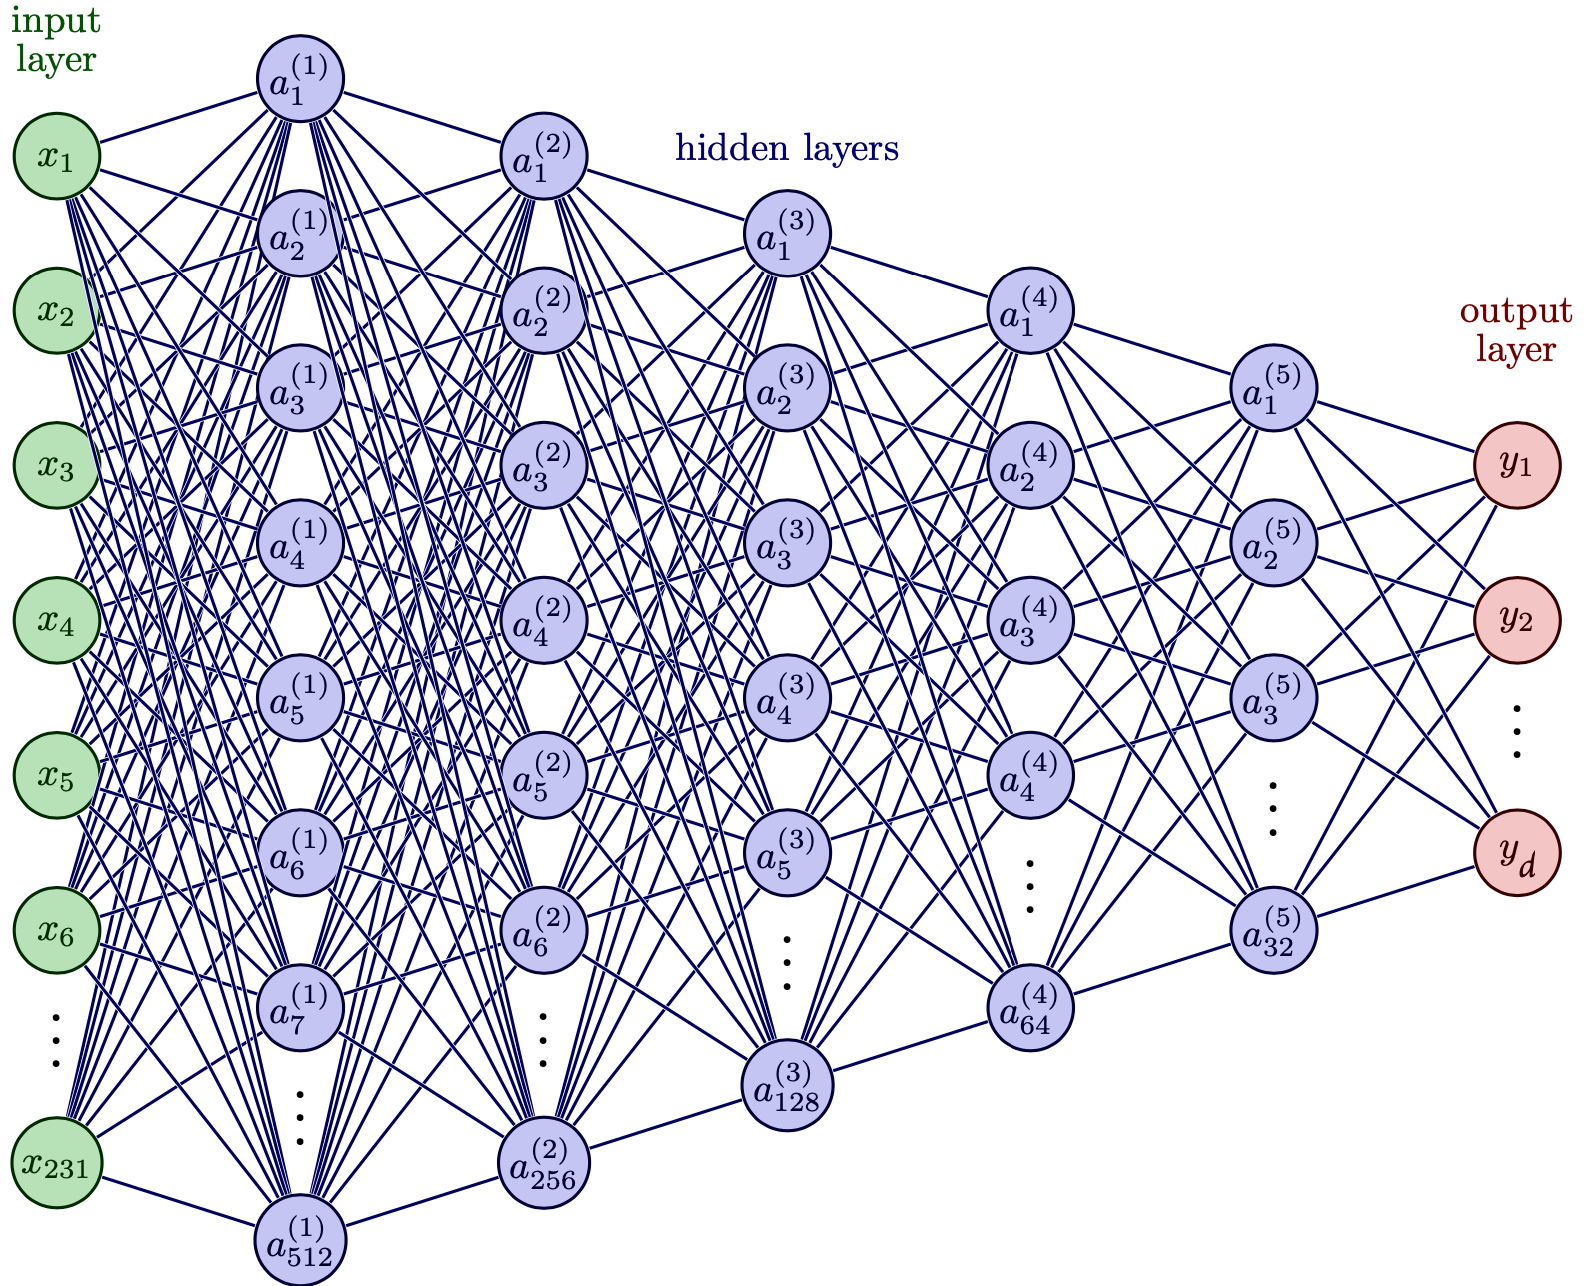
\includegraphics[width=\linewidth]{figures/NN_multiple_outputs.png}
    \caption{\textbf{Architecture of the Extended Feed-Forward Neural Network}. The input layer comprises 231 electrode recording input values, and the network outputs predicted $d$ target values depending on the specific problem to solve. The FFNN consists of five hidden layers. \\
    The vizualization has been made with Latex, with code adapteded from Neural Networks in TikZ with attribution to Izaak Neutelings and is licensed under the Creative Commons Attribution-ShareAlike 4.0 International License \cite{neutelings2021}.}
    \label{fig:NN_dipole_w_amplitude_architecture}
\end{figure}

In this extension of the FFNN, we continue to employ ReLU as the activation function in the input layer and the hyperbolic tangent for the hidden layers. This choice of architecture, combined with the selected hyperparameters, has consistently yielded promising results. The key difference in this extended network architecture is the integration of the Sigmoid activation function in the output layer. For an overview of the essential hyperparameters utilized to generate the forthcoming results in this extended model, please refer to Table \ref{tab:parameters}, which offers a summary of these overall elements.


\begin{table}
\centering
\begin{tabular}{|lc|}
\hline
\rowcolor[HTML]{CBCEFB}
\multicolumn{2}{|c|}{\cellcolor[HTML]{CBCEFB}{\color[HTML]{000000} \textbf{Extended FFNN}}}    \\ \hline
\rowcolor[HTML]{EFEFEF}
\multicolumn{1}{|l|}{\cellcolor[HTML]{EFEFEF}\textbf{Hyperparameters}} & \multicolumn{1}{l|}{\cellcolor[HTML]{EFEFEF}\textbf{Value}} \\ \hline
\multicolumn{1}{|l|}{Hidden layers}                                    & 5                                                           \\ \hline
\multicolumn{1}{|l|}{Optimizer}                                        & SGD                                                         \\ \hline
\multicolumn{1}{|l|}{Learning rate (initial)}                          & 0.001                                                       \\ \hline
\multicolumn{1}{|l|}{Momentum}                                         & 0.35                                                        \\ \hline
\multicolumn{1}{|l|}{Weight decay}                                     & 0.1                                                         \\ \hline
\multicolumn{1}{|l|}{Minibatch size}                                   & 32                                                          \\ \hline
\multicolumn{1}{|l|}{Dropout}                                          & 0.5                                                         \\ \hline
\multicolumn{1}{|l|}{Act.func in first layer}                           & ReLU                                                        \\ \hline
\multicolumn{1}{|l|}{Act.func in hidden layers}                         & Tanh                                                        \\ \hline
\multicolumn{1}{|l|}{Act.func in last layer}                           & Sigmoid                                                        \\ \hline
\end{tabular}
\caption{Hyperparameters for the Extended FFNN.}
\label{tab:parameters}
\end{table}


\rednote{This must come somewhere else?}
\subsection{Denormalization for Performance Evalutaion}
In this extended version of the fully connected feed-forward neural network (FCNN), assessing network performance through standard train-validation-loss plots becomes less informative due to the normalization of target values and a more complex cost function. Reading off unitless loss values from plots, where the cost function value is plotted against epochs, provides little insight beyond whether the network is capable of decreasing the loss with an increasing number of training iterations.

When evaluating the network's performance on the test data set, which still comprises 20,000 samples, it is therefore essential that the predictions outputted by the FFNN undergo denormalization. This enables us to facilitate a meaningful evaluation against the true target values. The denormalization process takes a straight forward approach, where we simply do the opposite operations from the once performed during normalization \ref{eq:scale_target}. The denormalized predicted value $\tilde{y}_{i,j}$ of the network is then given as:

% \begin{equation}
% y_i = \left(x_i + \text{min}(x)\right) \left(\text{max}(x) - \text{min}(x)\right)
% \label{eq:de_scale_target}
% \end{equation}
\begin{equation}
\tilde{y}_{i,j} = \biggl(\tilde{y}_{i,j}' + \text{min}(\{\tilde{\mathbf{y}}\}_j\biggr) \biggl(\text{max}(\{\tilde{\mathbf{y}}\}_j) - \text{min}(\{\tilde{\mathbf{y}}\}_j)\biggr).
\label{eq:de_scale_target}
\end{equation}

Here, $\tilde{y}_{i,j}' \in \mathcal{\tilde{Y}}'$ is the normalized target value for the $i$'th sample and the $j$'th dimension of the target vector , where $i \in \{0, N-1\}$ and $j \in \{0, d-1\}$. In the equation min($\{\tilde{\mathbf{y}}_j\}$) and max($\{\tilde{\mathbf{y}}_j\}$) denotes the minimum and maximum values for the specific target dimension across all samples.

%
% To comprehensively gauge the network's predictive abilities on this test dataset, we employ a diverse set of error metrics. While the primary focus is on minimizing the mean Euclidean distance of dipole positions and the absolute error for amplitude and radius, a range of other metrics are also explored for a comprehensive assessment. These metrics include mean absolute error (MAE), normalized mean absolute error considering the value range (NMAE), mean squared error (MSE), and root mean squared error (RMSE).


\section{Predicting Single Current Dipole Sources with Varying Magnitudes} \label{sec:result_magnitude}
\sectionmark{Single Current Dipoles with Magnitudes}

In this section, we introduce the concept of various magnitudes for single current dipole sources, which adds an additional dimension to the output of the FCNN, with $d=4$. Besides predicting the coordinates of the dipoles for each sample, the network now also estimates the magnitude of the dipole signals. In real-world scenarios, it might be of interest to not only pinpoint the location generating  abnormal brain activity but also comprehend the \emph{strength} of abnormality.By incorporating magnitude prediction into the network, we gain valuable insights into the problem at hand, allowing the network to extract more detailed information about the underlying brain activity from the EEG data.


\subsection{Adjusting Data Set}
For the purpose of this extended EEG inverse problem, the data set is modified by introducing varying magnitudes to each dipole, ranging from 1 to 10 nAm. This adjustment does not impact the number of features, which corresponds to the number of electrode recordings for each sample. However, it does increase the number of target values by 1. Figure \ref{fig:dipole_w_amplitude_example} showcases two examples from the data set, where the dipole's location remains constant while the magnitude of the dipole signal varies. We observe that the shape of the EEG signal remains consistent while the strength of the EEG signal is significantly higher for the dipole with the largest initiated magnitude, as intended.

It is important to note that this data set represents the data before the standardization procedure of the input data. However, scaling the EEG data ensures that each electrode measurement is uniformly affected, maintaining consistent relative differences in magnitude between weaker and stronger dipole signals.

\begin{figure}[!htb]
    \centering
    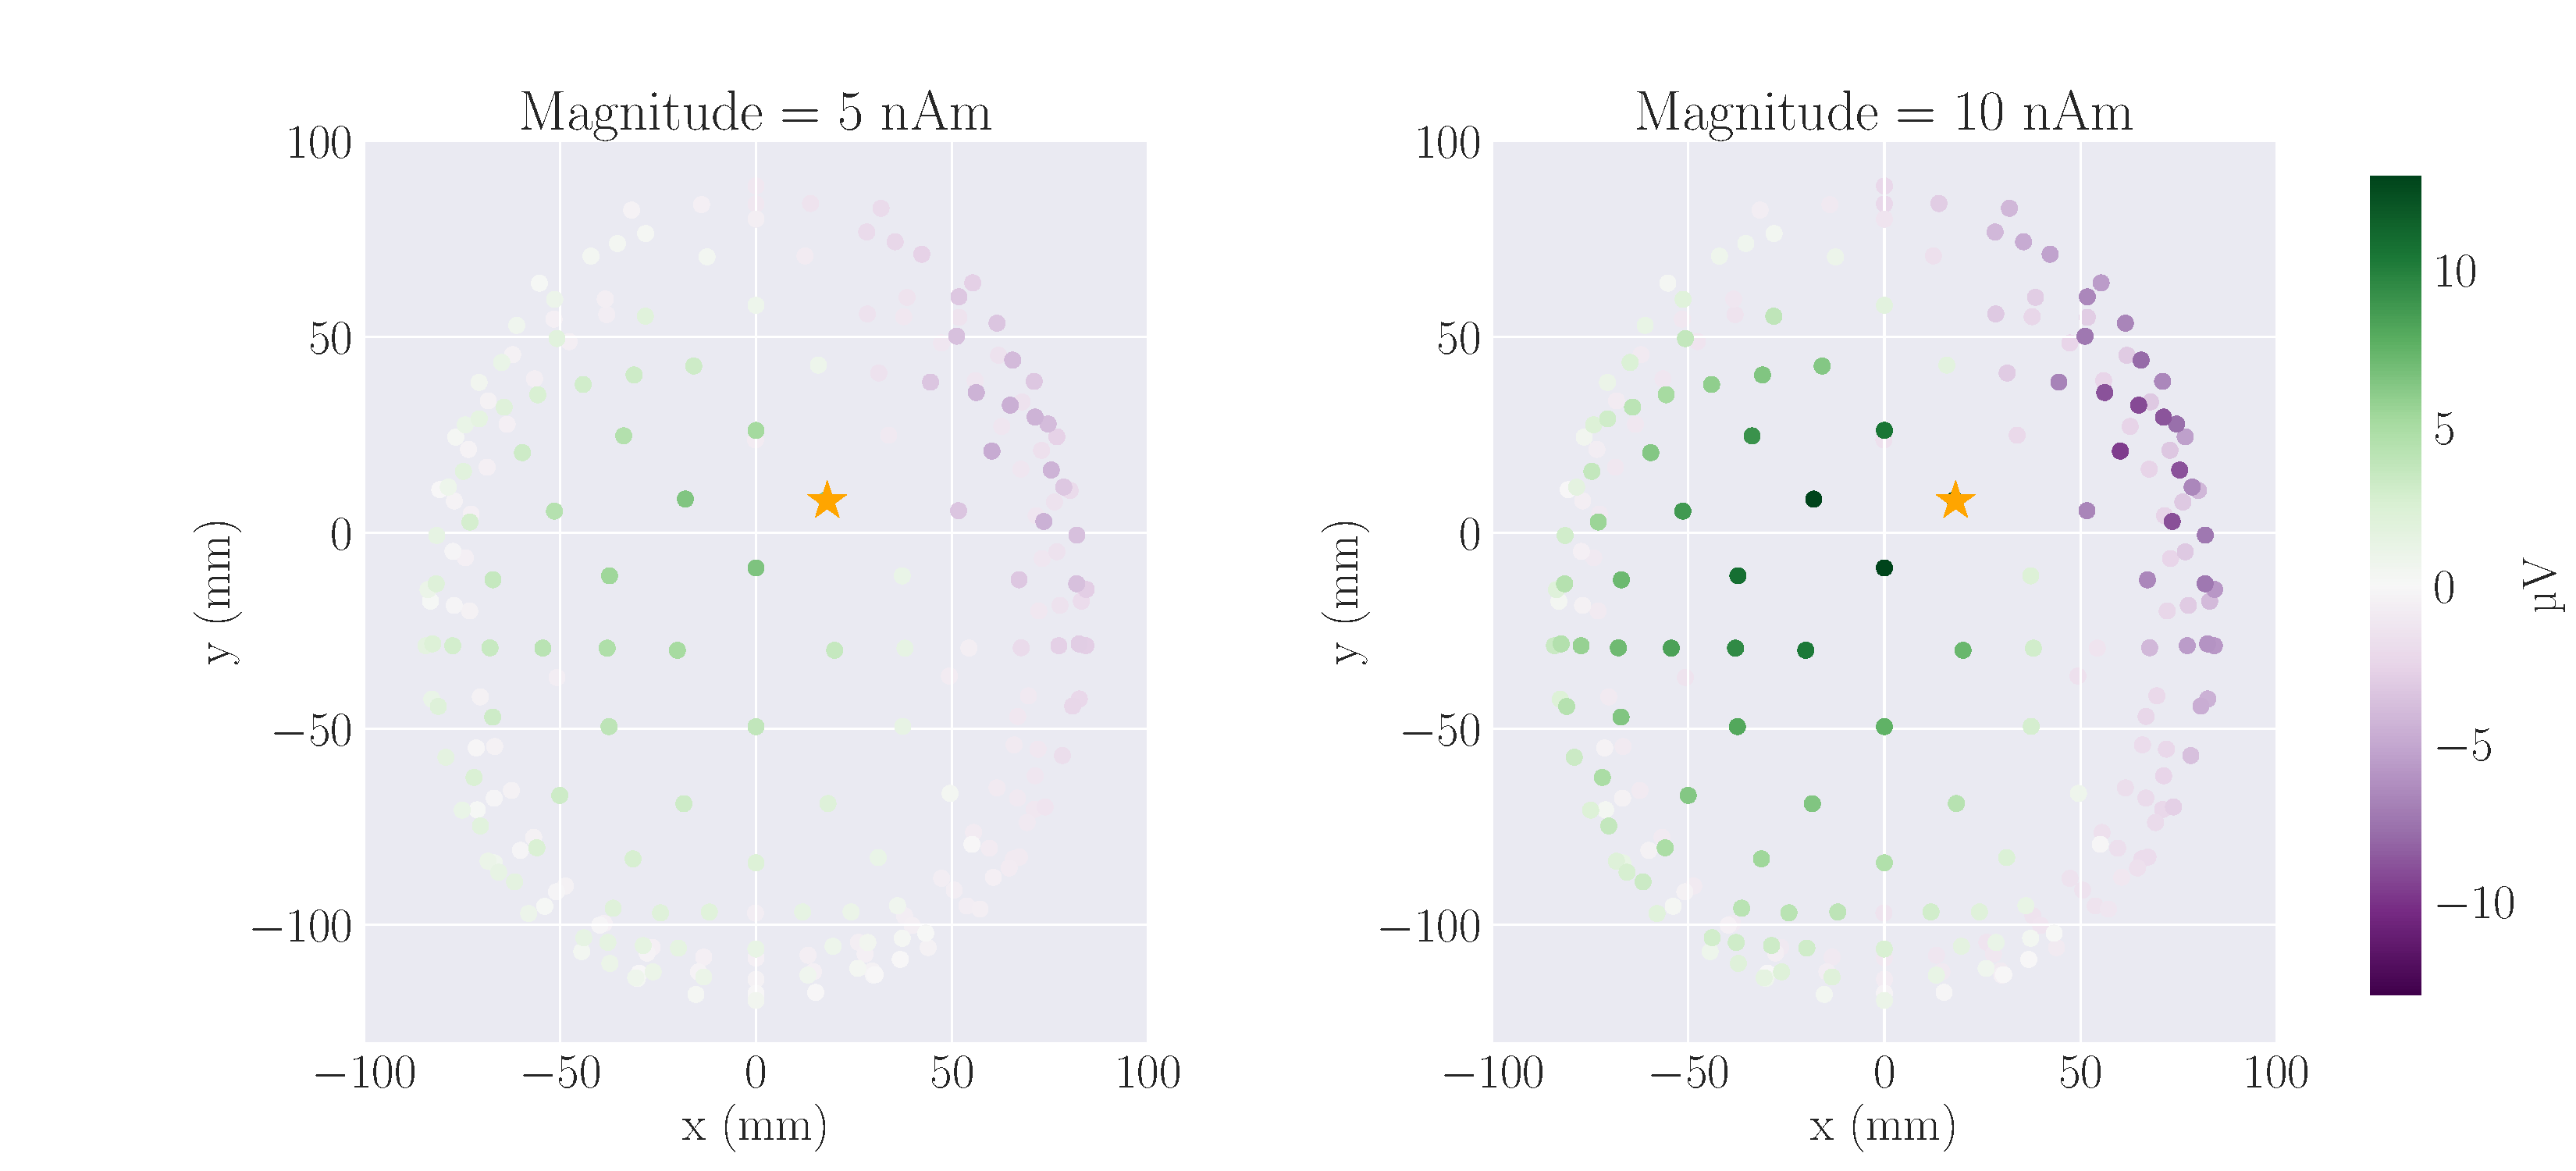
\includegraphics[width=\linewidth]{figures/purple_green/dipole_w_amplitude_example.pdf}
    \caption{EEG data for two samples with current dipole magnitudes equal to 5 and 10 nAm, respectively. The EEG recordings have a range between -10 and 10 $\mu$V.}
    \label{fig:dipole_w_amplitude_example}
\end{figure}


\subsection{Performance Evaluation}
To assess the network's performance, we start by analyzing the accuracy in relation to training epochs, as depicted in Figure \ref{fig:dipole_w_amplitude_loss}. We emphasize that it is important to note that the target values have been normalized, resulting in unitless loss measurements. Therefore, the figure provides a qualitative representation of the network's training progress rather than precise loss values. The plot clearly demonstrates a consistent pattern of decreasing loss as the number of epochs increases, indicating that the network is able to capture underlying patterns in the data. Moreover, both the training and validation loss stabilize after approximately 1100 epochs, suggesting that the network has reached its optimal performance level. Each epoch takes about 20 seconds to finish, leaving us with a training time of roughly 8.5 hours in total.

\begin{figure}[!htb]
    \centering
    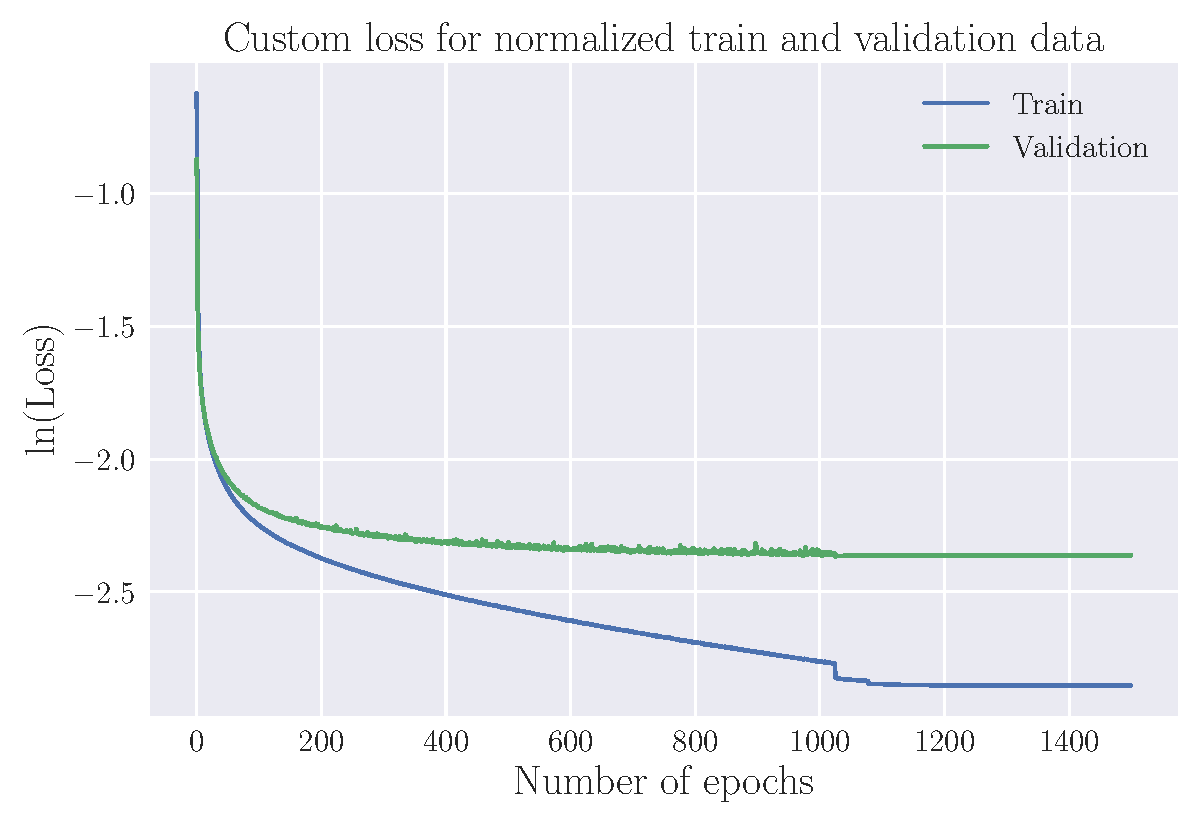
\includegraphics[width=\linewidth]{figures/NN_magnitude/Custom_Loss_amplitudes_test_custom_loss_tanh_32_0.001_0.35_0.1_0_1500_(0).pdf}
    \caption{Training and validation loss as functions of epochs for the extended FFNN model, which predicts both location and magnitude parameters. The analysis is based on simulated data comprising 50,000 samples and spans a training duration of 1500 epochs.}
    \label{fig:dipole_w_amplitude_loss}
\end{figure}

In Figure \ref{fig:dipole_w_amplitude_targets}, we present the progression of the loss for the target parameters. Notably, after approximately 1100 epochs, the loss stops fluctuating for all target values, suggesting potential full convergence at this stage. It is evident that the loss for the magnitude target converges at a higher value, compared to the target coordinates. The $x$-, $y$-, and $z$-coordinate targets gradually converge to values that closely align with one another. Among these, the $y$-coordinate achieves the lowest loss, followed by the $x$-coordinate, and then the z-coordinate.

\begin{figure}[!htb]
    \centering
    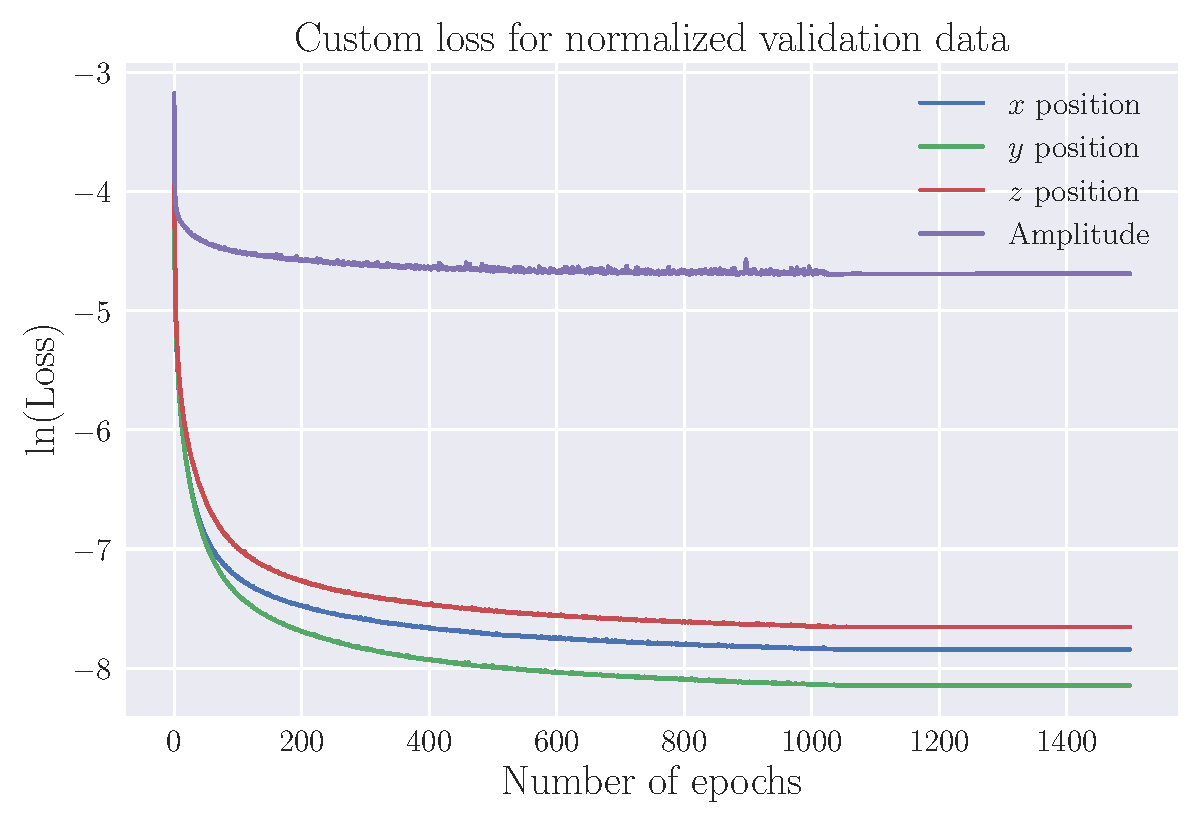
\includegraphics[width=\linewidth]{figures/NN_magnitude/Custom_Loss_mse_targets_amplitudes_test_custom_loss_tanh_32_0.001_0.35_0.1_0_1500_(0).pdf}
    \caption{Validation loss as a function of epoch for each target value, including the $x$-, $y$-, and $z$-coordinates of the dipole, as well as the magnitude of the dipole signal.}
    \label{fig:dipole_w_amplitude_targets}
\end{figure}

%Considering the range associated with each coordinate profile, we observe that the MAE for the $x$ coordinate, at 1.348 mm, accounts for only 0.936$\%$ of the complete range. Similarly, for the $y$-coordinate, exhibiting a MAE of 1.448 mm, the error relative to the coordinate range stands at 0.809$\%$. Lastly, the $z$ coordinate, with a MAE of 1.411 mm, represents 1.052$\%$ of the full range. This balanced distribution of errors suggests that no single dimension to a large extent exhibits higher error propensity than the others, thereby indicating robust overall performance. As observed in the network's performance when predicting single current dipoles with constant magnitudes, the $z$ coordinate consistently exhibits the largest error. This suggests the potential presence of specific challenges in predicting this dimension.

%MSE, due to its quadratic nature, penalizes larger errors more prominently. Despite this, the MSE values remain within reasonable bounds when contextualized within the coordinate ranges, implying a stable error profile with few significant outliers. This is a satisfying finding, especially considering the narrower range of the magnitude target. However, it is important to recognize that the theoretical lower limit of MSE is always 0, which means there is still room for further improvement in accurately capturing variations in all the target values.

%This represents a value more than 100$\%$ larger than the MED obtained when the FFNN predicted only the dipole locations for dipoles with a constant magnitude of electrical signal. Nevertheless, it is crucial to underscore that, given the dimensions of the brain within the NYHM, and the theshold value we aim to laty under, this error is relatively small and satisfactory.


In Table \ref{table:error_simple_dipole}, we present the network's performance across various target categories using different error metrics. Analyzing the outcomes pertaining to the target coordinates reveals a noteworthy consistency in mean absolute error, with an average deviation of less than 1.5 mm from the true values. In contrast to when studying single dipoles with constant strength, the $z$-coordinate stands for the highest contribtuion to this MAE. The MAE for the magnitude variable equals 0.539 nAm. Having that the magnitude range spans from 1 to 10 nAm, this error translates to a relative error of 6.00$\%$. In other words, the network's predictions for the magnitude variable are, on average, within 6.00$\%$ of the true values within this range.

In addition to MAE, we look into the network's performance through the metrics of mean squared error and root mean squared error, which offer complementary insights. For the $x$-coordinate, the MSE stands at 3.438 mm$^2$, while for the $y$- and $z$-coordinate, it is 3.860 mm$^2$ and 3.862 mm$^2$, respectively. The MSE for the magnitude target, measures 0.650 nA$^2$m$^2$.

The Root Mean Squared Error, which indicates the standard deviation of prediction errors and their distribution around the mean, reports values slightly lower than the corresponding Mean Squared Error values. Specifically, RMSE values measure at 1.854 mm, 1.965 mm, and 1.965 mm for the distinct target coordinates, and 0.806 nAm for the magnitude target. These RMSE values suggest that, on average, the prediction errors align with the overall spread of errors, without significant outliers or extreme deviations from the mean error. This indicates a level of stability and predictability in the error distribution.



\begin{table}[!htb]
\begin{tabular}{l|
>{\columncolor[HTML]{FFFFFF}}c
>{\columncolor[HTML]{FFFFFF}}c
>{\columncolor[HTML]{FFFFFF}}c
>{\columncolor[HTML]{FFFFFF}}c
>{\columncolor[HTML]{FFFFFF}}c |}
\cline{2-6}
                                                   & \multicolumn{5}{c|}{\cellcolor[HTML]{CBCEFB}\textbf{Error Metrics for Target Values}}                                                                                                                                                                                                                                                                                                                                                                                                                                                                                            \\ \cline{2-6}
                                                   & \multicolumn{1}{l|}{\cellcolor[HTML]{EFEFEF}\begin{tabular}[c]{@{}l@{}}x-coordinate\\ {[}mm{]}\end{tabular}} & \multicolumn{1}{l|}{\cellcolor[HTML]{EFEFEF}\begin{tabular}[c]{@{}l@{}}y-coordinate\\ {[}mm{]}\end{tabular}} & \multicolumn{1}{l|}{\cellcolor[HTML]{EFEFEF}\begin{tabular}[c]{@{}l@{}}z-coordinate\\ {[}mm{]}\end{tabular}} & \multicolumn{1}{l|}{\cellcolor[HTML]{EFEFEF}\begin{tabular}[c]{@{}l@{}}Position \\ Error {[}mm{]}\end{tabular}} & \multicolumn{1}{l|}{\cellcolor[HTML]{EFEFEF}\begin{tabular}[c]{@{}l@{}}Magnitude\\ {[}nAm{]}\end{tabular}} \\ \hline
\multicolumn{1}{|l|}{\cellcolor[HTML]{EFEFEF}MAE}  & \multicolumn{1}{c|}{\cellcolor[HTML]{FFFFFF}1.348}                                                           & \multicolumn{1}{c|}{\cellcolor[HTML]{FFFFFF}1.448}                                                           & \multicolumn{1}{c|}{\cellcolor[HTML]{FFFFFF}1.420}                                                           & \multicolumn{1}{c|}{\cellcolor[HTML]{FFFFFF}1.405}                                                                  & 0.539                                                                                                           \\ \hline
\multicolumn{1}{|l|}{\cellcolor[HTML]{EFEFEF}MSE}  & \multicolumn{1}{c|}{\cellcolor[HTML]{FFFFFF}3.438}                                                          & \multicolumn{1}{c|}{\cellcolor[HTML]{FFFFFF}3.860}                                                          & \multicolumn{1}{c|}{\cellcolor[HTML]{FFFFFF}3.862}                                                          & \multicolumn{1}{c|}{\cellcolor[HTML]{FFFFFF}3.720}                                                                 & 0.650                                                                                                           \\ \hline
\multicolumn{1}{|l|}{\cellcolor[HTML]{EFEFEF}RMSE} & \multicolumn{1}{c|}{\cellcolor[HTML]{FFFFFF}1.854}                                                           & \multicolumn{1}{c|}{\cellcolor[HTML]{FFFFFF}1.965}                                                           & \multicolumn{1}{c|}{\cellcolor[HTML]{FFFFFF}1.965}                                                           & \multicolumn{1}{c|}{\cellcolor[HTML]{FFFFFF}1.929}                                                                  & 0.806                                                                                                           \\ \hline
\end{tabular}
\caption{\textbf{Evaluation of the extended FFNN's performance utializing different Error Metrics.} \newline
Performance for the extended FFNN on test data set consisting of 1000 samples. The errors are measured using Mean Squared Error (MSE), Mean Absolute Error (MAE), and Root Mean Squared Error (RMSE).}
\label{table:error_simple_dipole}
\end{table}

In Figure \ref{fig:magnitude_errors}, we present the AE and SE metrics calculated between predicted and target coordinate values as a function of the magnitude of the dipole strengths. The figures reveal a relatively higher occurance of outliers when the magnitude of the dipole strength is small, with elevated AE and SE values. This trend may initially suggest that the neural network encounters greater challenges in accurately predicting the positions of dipoles with smaller magnitudes. However, we cannot rule out that these disparities might be related to alternative factors such as depth positioning, intricate cortical folding patterns, or other random fluctuations.

When examining the correlation coefficients for each of the figures, we find that the correlation between the strength of the dipole and the error in position prediction has a correlation of -0.01 and -0.02 for the AE and SE, respectively. These correlation coefficients do suggest a negative correlation (decreasing error with increasing magnitudes), but their values are nearly zero, indicating a weak linear relationship. Upon closer inspection of the figure, keeping in mind that it contains 20,000 scatter points, we notice that most of the predictions exhibit an AE smaller than 5 nAm and an SE smaller than 10 nA$^2$m$^2$. This suggests that, despite observed variations in predictions for samples with smaller magnitudes, the majority of the FFNN's positional predictions consistently cluster within this range of lower errors.

\begin{figure}
  \hspace*{-2.5cm} % Adjust the value as needed to move the figures left
  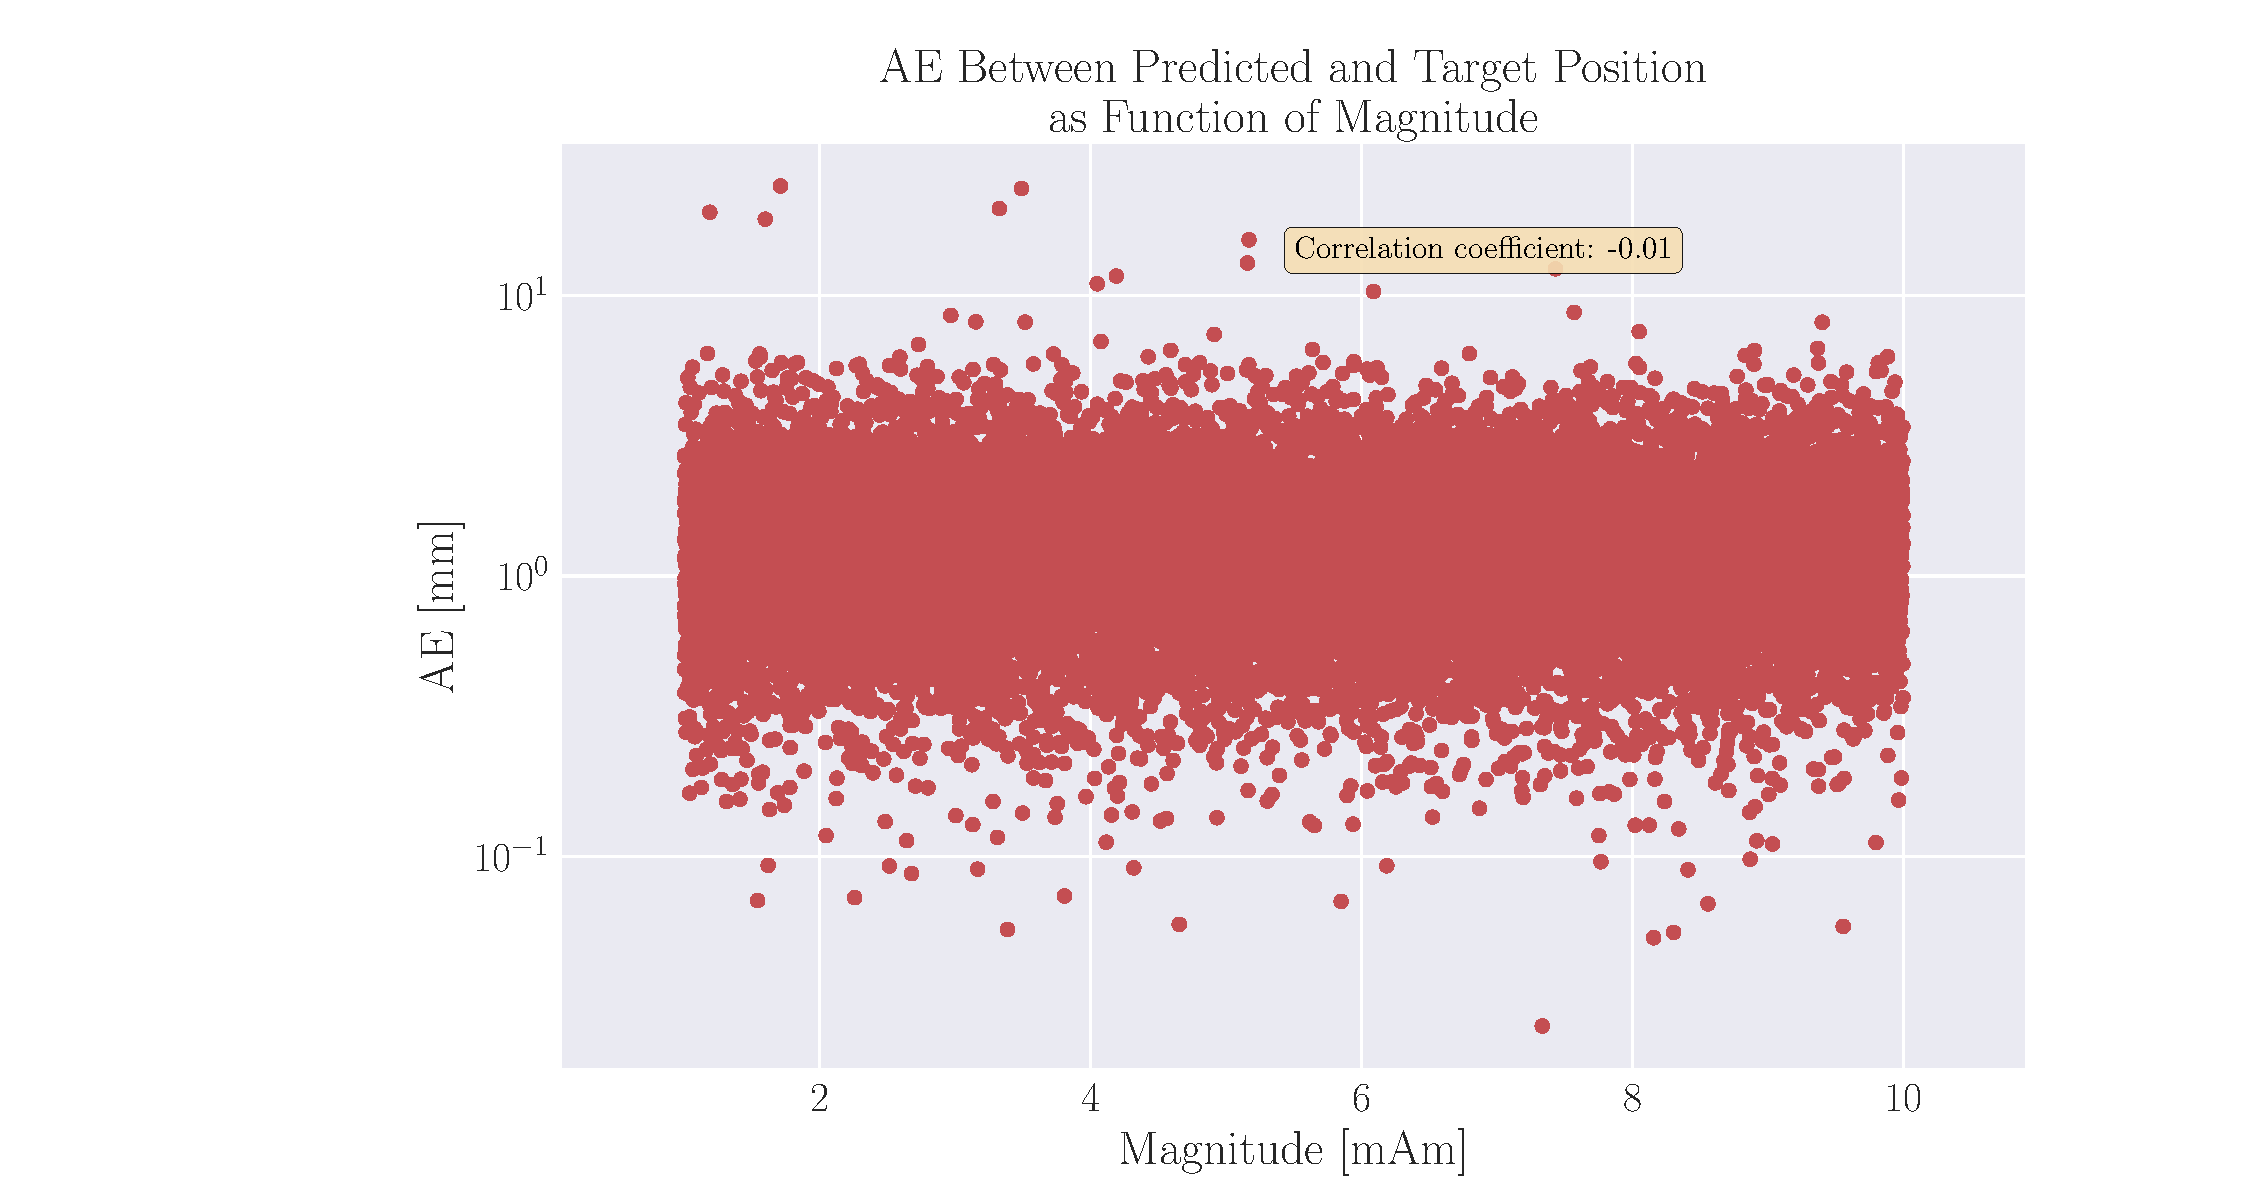
\includegraphics[width=9cm]{figures/mae_amplitude0.pdf}
  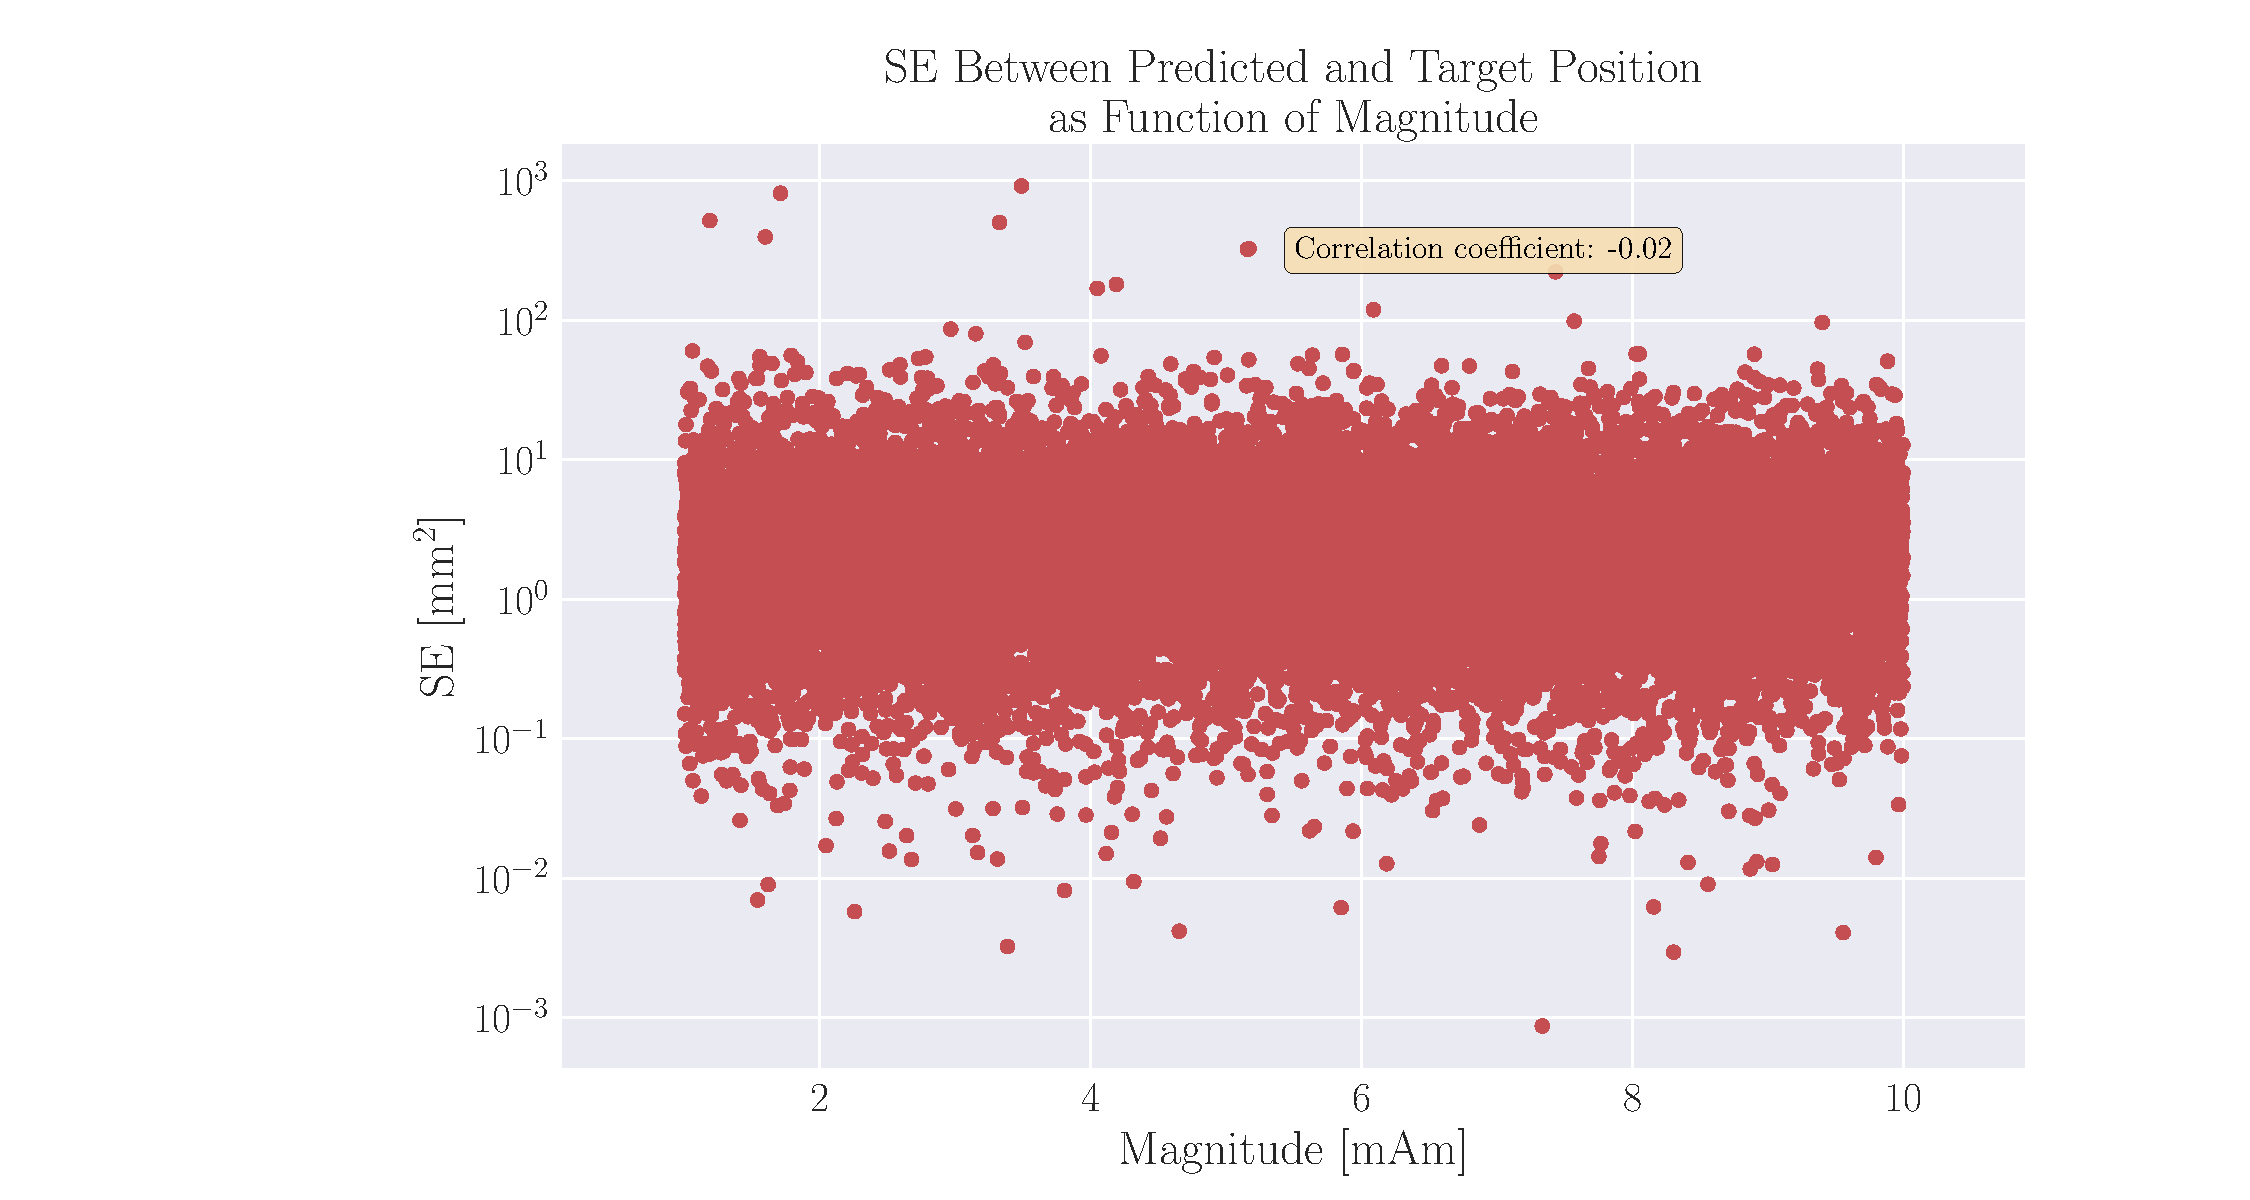
\includegraphics[width=9cm]{figures/mse_amplitude0.pdf}
  \caption{Scatter plot of Abolsute Error and Squared Error computed between predicted and target coordinate values, as function of the magnitude of the dipole strengths.}
  \label{fig:magnitude_errors}
\end{figure}

The Mean Euclidean Distance of the FFNN's predictions on the unseen test data is measured at 2.815 mm. Table \ref{table:MED_magnitude} presents the percentages of predictions of test samples falling within various MED threshold values. Notably, the network achieves an accuracy smaller than 12 mm for 99.8$\%$ of the test data. Furthermore, 64.3$\%$ of the samples exhibit a MED smaller than 3 mm, an achievement that, while robust, falls slightly short of the FFNN's performance in the previous, less complex problem.

\begin{table}[]
  \centering
\begin{tabular}{|ccc|}
\hline
\rowcolor[HTML]{CBCEFB}
\multicolumn{3}{|c|}{\cellcolor[HTML]{CBCEFB}\textbf{Euclidian Distance for Test Samples}}                                                             \\ \hline
\rowcolor[HTML]{EFEFEF}
\multicolumn{1}{|c|}{\cellcolor[HTML]{EFEFEF}ED \textless 5 mm} & \multicolumn{1}{c|}{\cellcolor[HTML]{EFEFEF}ED \textless 10 mm} & ED \textless 15 mm \\ \hline
\rowcolor[HTML]{FFFFFF}
\multicolumn{1}{|c|}{\cellcolor[HTML]{FFFFFF}90.930 $\%$}       & \multicolumn{1}{c|}{\cellcolor[HTML]{FFFFFF}99.505 $\%$}        & 99.925 $\%$        \\ \hline
\end{tabular}
\caption{\textbf{ED between targets and predictions of test samples; Predicting Location and Magnitude with the FFNN} \newline
Performance of the FFNN on the test dataset comprising 20,000 samples, presented as the percentage of samples falling within ED thresholds of 5 mm, 10 mm and 15 mm respectively.}
\label{table:MED_magnitude}
\end{table}

Figure \ref{fig:histogram_magnitude} displays two panels, depicting the ED between predicted and true target coordinates and AE between predicted and true magnitude of each test sample within bins of width 1 unit. In the left panel, representing the ED histogram, the bins corresponding to ED values of 2 and 3 mm are the most populated, containing the largest proportion of samples. This panel also illustrates that the majority of predicted locations for the test samples exhibit a ED error smaller than 14 mm.

Turning our attention to the right panel, which displays the AE for predicted magnitudes, we observe that the bin holding samples with a magnitude prediction AE less than 1 nAm holds the most samples. Within this bin, 17,014 out of the 20,000 samples can be found, signifying that the network predicts the magnitude with a AE smaller than 1 nAm for approximately 85$\%$ of the sample set.

\begin{figure}
  \hspace*{-2.8cm} % Adjust the value as needed to move the figures left
  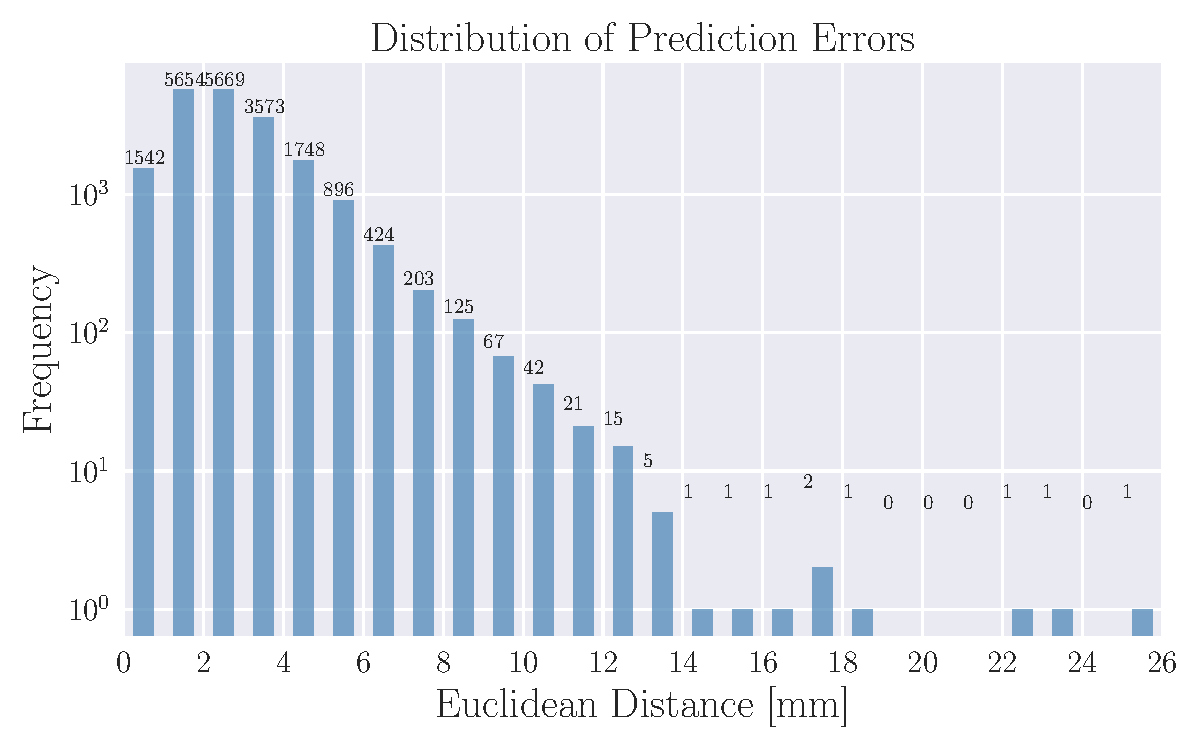
\includegraphics[width=9cm]{figures/new_histogram_position_amplitude.pdf}
  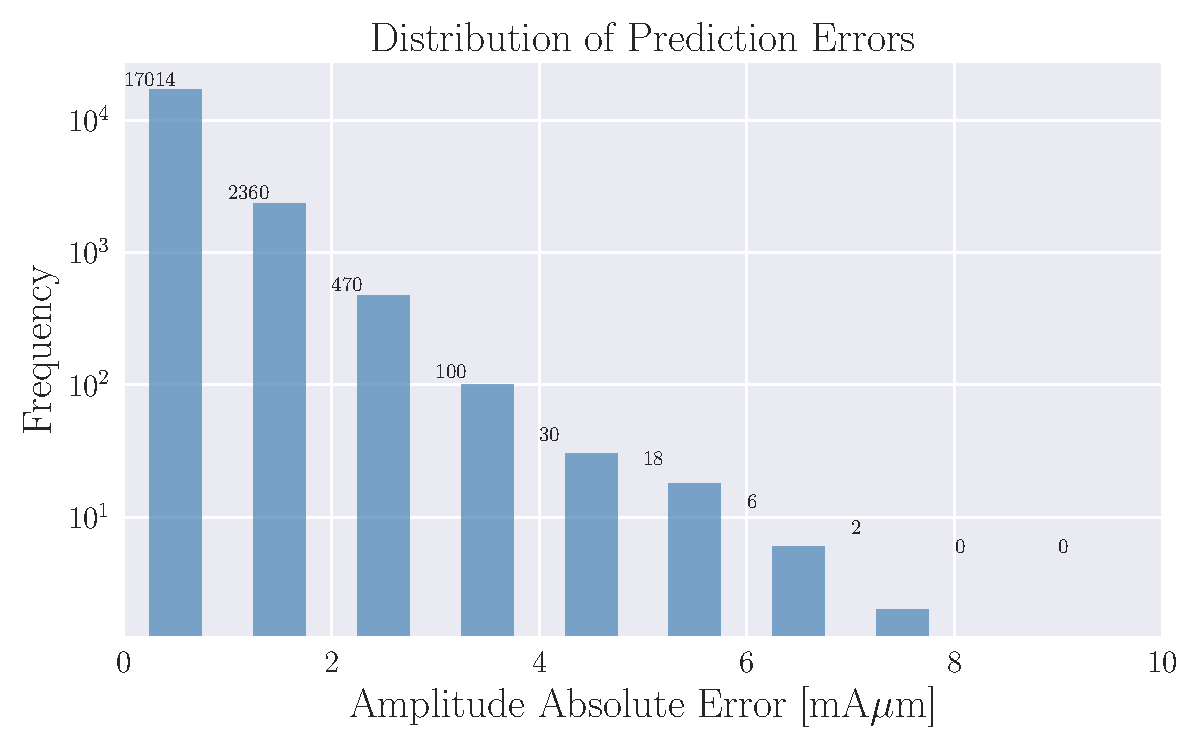
\includegraphics[width=9cm]{figures/new_histogram_amplitude_amplitude.pdf}
  \caption{Left panel illustrates the distribution of Mean Euclidean Distance for the predicted dipole locations, organized into bins of width 1 mm. Right panel holds the distribution of Mean Absolute Error for the predicted magnitude of dipole electrical signal, presented in a similar format, with bins of width 1 nAm.}
  \label{fig:histogram_magnitude}
\end{figure}


\section{Predicting Region of Active Correlated Current Dipoles with Magnitudes} \label{sec:result_area}
\sectionmark{Population of Current Dipoles with Magnitudes}
\rednote{Kan jeg omtale populasjonene som sfæriske?}
In this problem we expand the data set for the FFNN to include varying radii and magnitudes for the origins generating the electrical activity detected by the recording electrodes. In this extension, the FFNN progresses from predicting the location and magnitude of individual current dipole moments to estimating the centers of larger spherical populations. This enhancement aims to enable the network to extract more detailed information from EEG data, which could be valuable in scenarios where understanding the extent of brain abnormalities is crucial.

\subsection{Adjusting Data Set}
In order to optimize the neural network's capacity for predicting dipole population regions, we made specific adjustments to the data set. Within this framework, each dipole population comprises individual dipoles distributed across all points within the NY head cortex falling within a spherical volume ranging from 1 mm to 15 mm in radius. Notably, guidelines established by Delucchi et al. (1962)\cite{delucchi1962scalp}, Cooper et al. (1965)\cite{cooper1965comparison}, Ebersole (1997)\cite{ebersole1997defining}, Nunez and Srinivasan (2006)\cite{nunez2006electric}, and Schomer and Lopes da Silva (2018)\cite{niedermeyer2005electroencephalography} in the clinical context of spontaneous EEG, suggest that for EEG recordings to detect brain activity, approximately 6-10 cm$^2$ of contiguous brain tissue must exhibit synchronous activity. A spherical radius of 15 mm translates to an approximate area of 7 cm$^2$, and thus falls within this criterion \cite{nunez2019multi}.

However, in event-related potentials (ERPs) experiments, which is what we think our simulated EEG data represents, a different perspective emerges. In ERPs the brain's responses to specific stimuli is investigated and in order to enhance the reliability of these responses, trial-averaging is a common practice, as outlined in Chapter \ref{chap:eeg_data}. Consequently, as suggested by these authors, it becomes plausible that EEG activity arising from brain regions smaller than the typical 6-10 cm$^2$ criterion for spontaneous EEG could be detectable - population sizes that we will be training our network to identify.

However, in the context of event-related potentials (ERPs) experiments, which is how our simulated EEG data can be considered, a different perspective arises. ERPs investigate the brain's responses to specific stimuli, and to enhance the reliability of these responses, trial-averaging is a common practice, as outlined in Chapter \ref{chap:eeg_data}. Consequently, as suggested by these authors, it becomes plausible that EEG activity arising from brain regions smaller than the typical 6-10 cm$^2$ criterion for spontaneous EEG could be detectable — population sizes that we will be training our network to identify.

For simplification reasons, we maintain the maximum amplitude strength of the total populations at 10 nAm. Consequently, we calculate the maximum number of points within a volume sphere with a radius of 15 mm and reduce this number by 10 in order to determine the strength of a distinct dipole within a given area. Having that the maximum number of dipoles that fit within a volume sphere with an ideal center and radius 15 mm was 899 dipoles, we were left with a dipole strength of 10/899 nAm for each dipole. The strength of a dipole population is thus directly proportional to the radius of the dipole population. While this may not perfectly represent real-world scenarios, it provides a reasonable approximation for our model.

In Figure \ref{fig:dipole_area}, we present an example of a dipole population and the corresponding EEG signal. The upper panels show the EEG signals for the specific sample, seen from different angels. The recording electrode locations are presented as filled circles, where the color of the fill represents the amplitude of the measured EEG signal for the given electrode. The yellow filled circles in the plots in the lower panel represents the diple populations, i.e. positions within the cortex where dipoles have been placed. The plots within the figure are seen from the $xz$-plane, $xy$-plane, and $yz$-plane.

\begin{figure}[!htb]
\centering
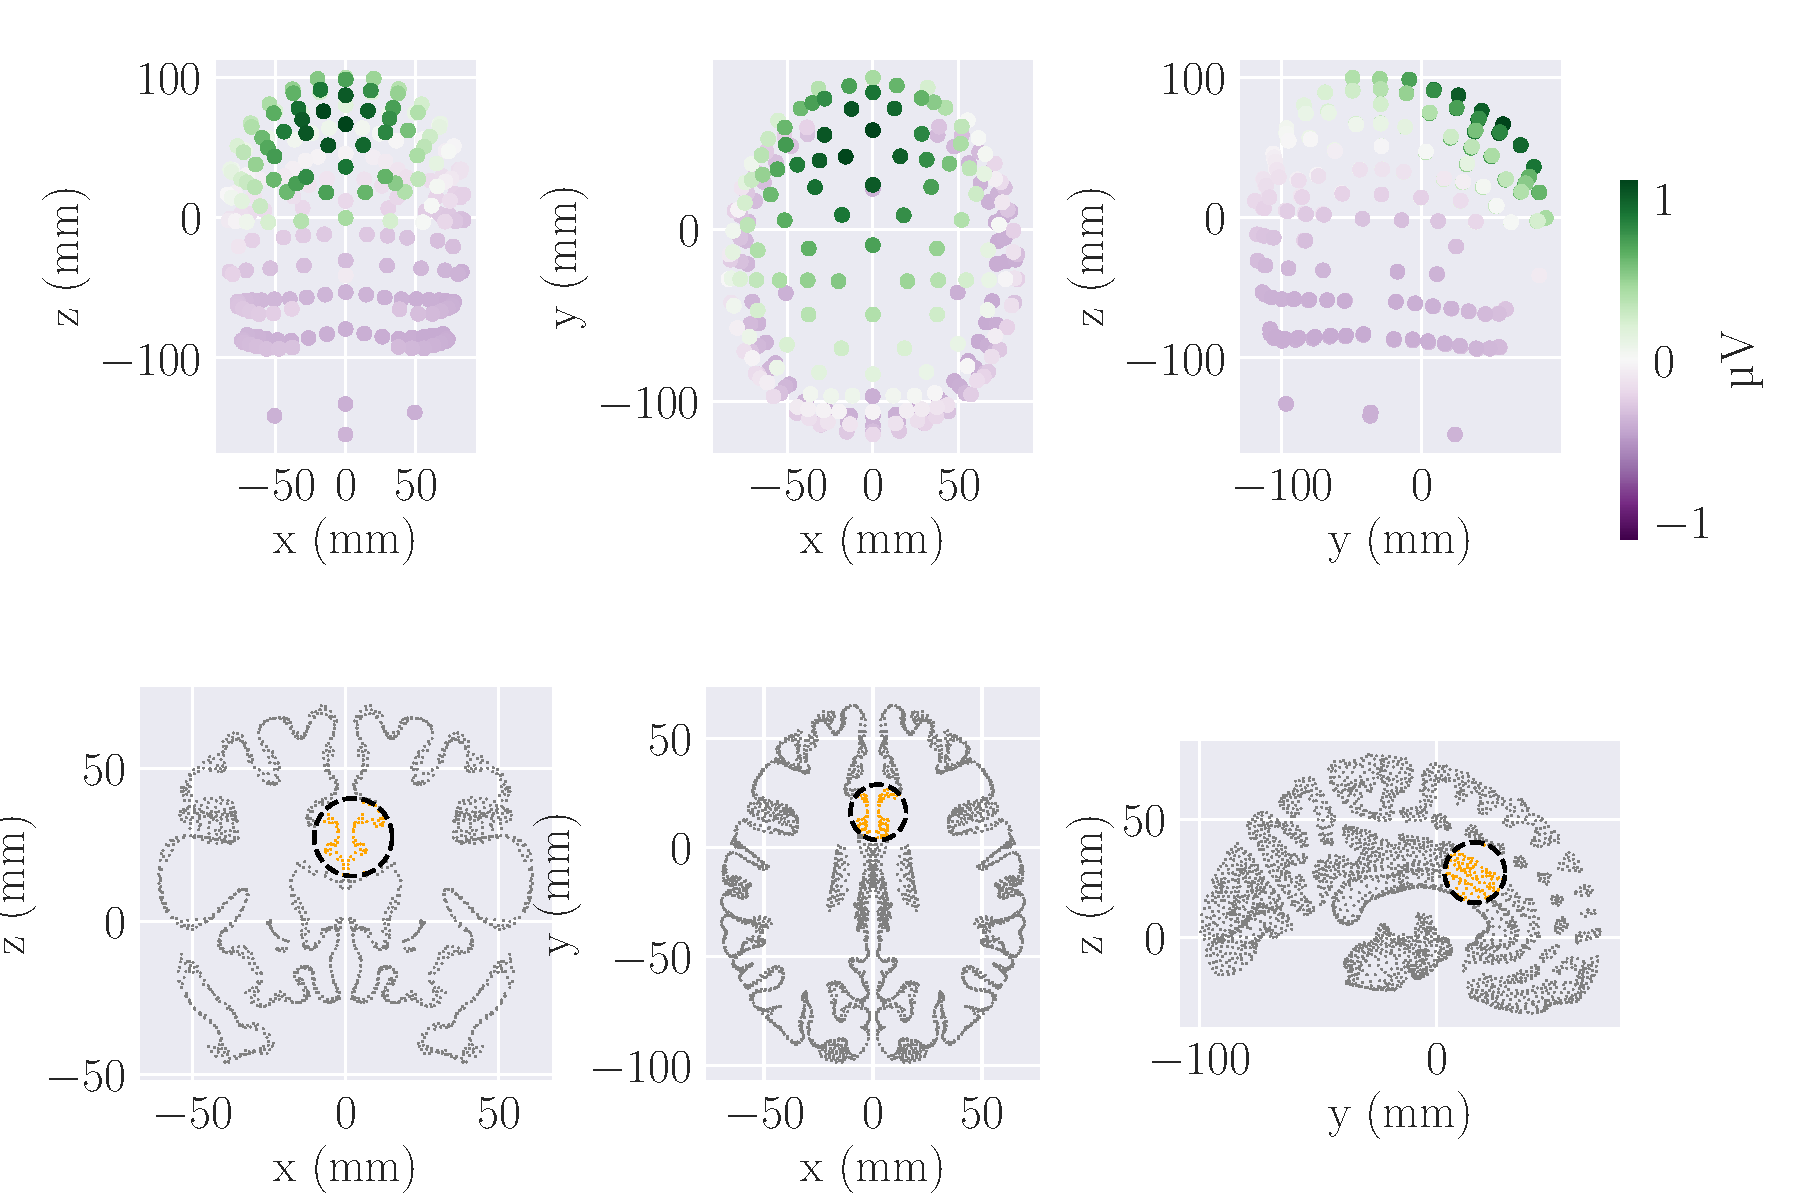
\includegraphics[width=\linewidth]{figures/purple_green/dipole_area_reduced_0.pdf}
\caption{EEG for a sample containing a spherical population of current dipole sources with a random center within the cerebral cortex.
\textbf{Upper panels:}
The EEG measure is seen from the front ($xz$-plane), side ($yz$-plane), and top ($xy$-plane) of the cortex. EEG electrode locations are presented as filled circles, where the color of the fill represents the amplitude of the measured signal for the given electrode.
\textbf{Lower panels:}
Gray filled circles represent points within the NY cortex where a dipole could have been placed. Yellow filled circles represent positions within the cortex where dipoles have been placed.}
\label{fig:dipole_area}
\end{figure}

% \rednote{Place somewhere else if needed?}
% As for the dataset, the number of target values is now 5: x, y, z-coordinates of the center of the dipole population, total magnitude, and radius. The number of features within the dataset is not modified and still holds 231 values, representing the EEG signal measured at every recording electrode.

% \begin{figure}[!htb]
% \centering
% 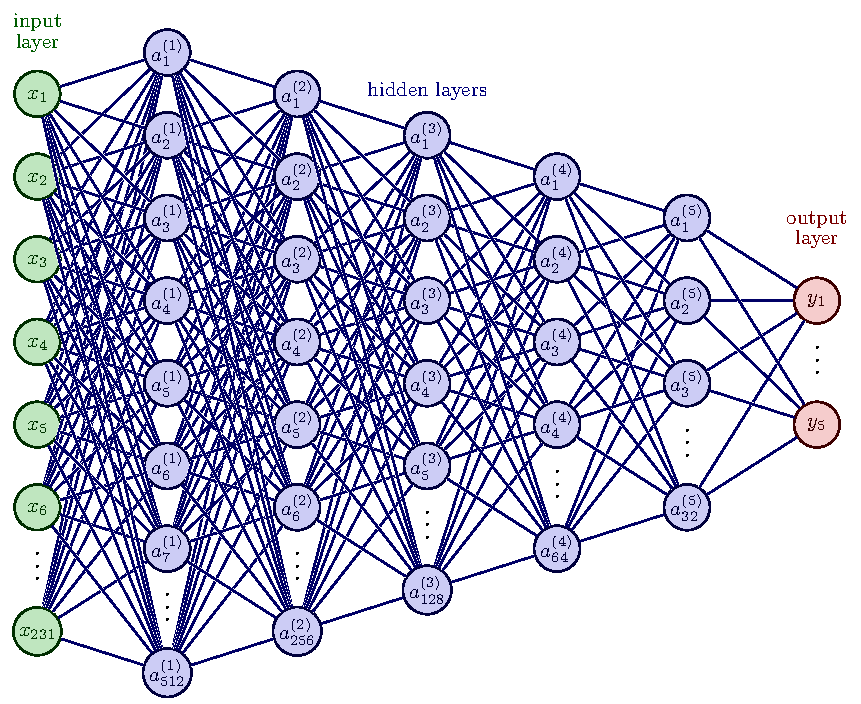
\includegraphics[width=\linewidth]{figures/NN_dipole_area_architecture.pdf}
% \caption{Architecture of the dipole area prediction network.}
% \label{fig:NN_dipole_area_architecture}
% \end{figure}

% \rednote{Rewrite/remove}
% Similar to the previous problem, we normalize the target values to ensure they all range from 0 to 1. Moreover, in this extension of the DiLoc network, we use the same activation functions as in the previous problem with ReLU as the activation function in the first layer, hyperbolic tangent for the hidden layers, and the Sigmoid activation function in the output layer.
%As with the previous problems, we have explored various network architectures and activation functions, but the current configuration has shown the best performance in terms of accurate predictions for this problem. It is important to emphasize that our primary goal is to find a network that can effectively solve the problem and provide accurate predictions, rather than necessarily seeking the best possible configuration.


\subsection{Performance Evaluation}
% How does the loss relate to size of population
% Exammple run and how long time it takes to calculate

In Figure \ref{fig:dipole_area_result}, we present the training and validation costumized loss for the FFNN as a function of epochs. We once again emphasize that the network's loss is unitless, meaning that the figure only provides a visual representation of the network's training progress rather than directly interpretable loss values. The network was trained for 1000 epochs. We see a clear trend of decreasing loss with an increasing number of epochs. However, after epoch 800, both training and validation loss appears to reach convergence, and beyond this point, there is no further improvement in loss. We can therefor conclude that overfitting has not taken place during training. At epoch 749, the learning rate is adjusted from 0.001 to 0.00004, resulting in a noticeable reduction and stabilization for both training and validation loss. On average, each epoch takes approximately 23 seconds to complete, resulting in a total training time of approximately 9.5 hours.


\begin{figure}[!htb]
    \centering
    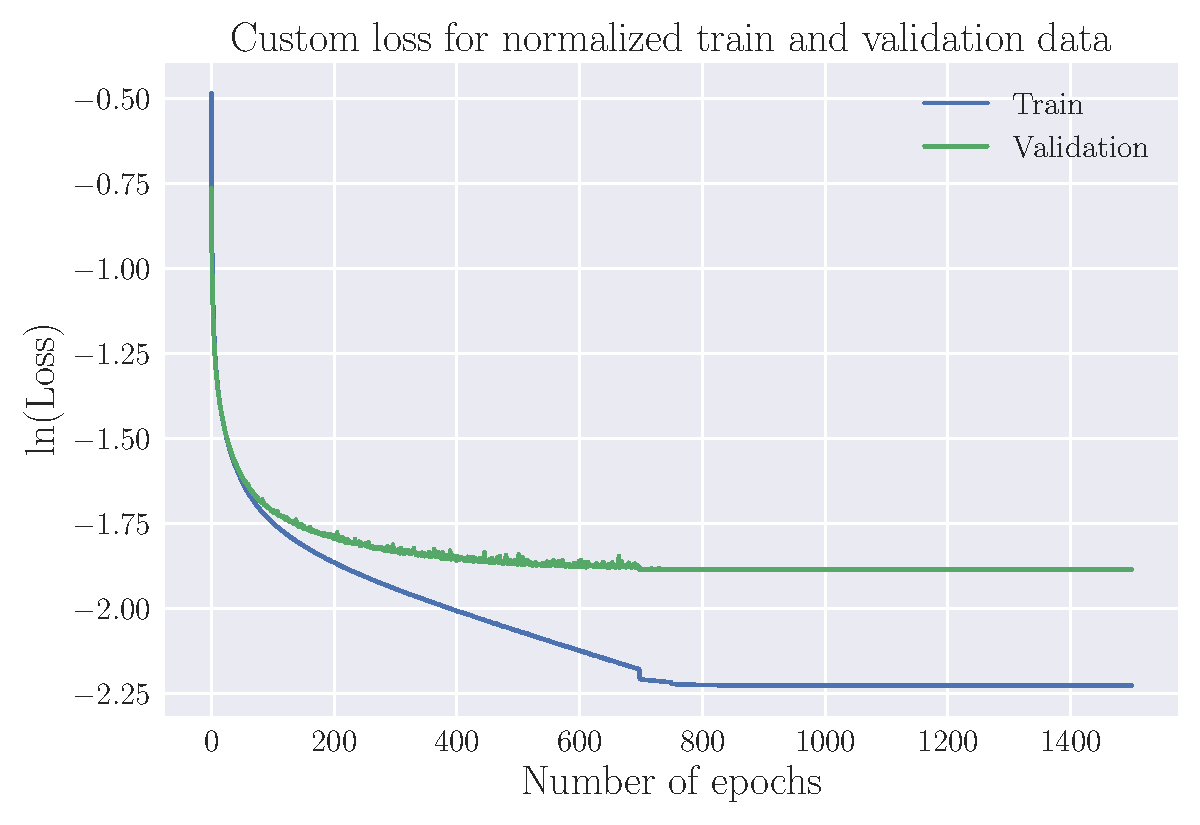
\includegraphics[width=\linewidth]{figures/NN_area/Custom_Loss_area_seed_42_cnn_32_0.001_0.35_0.1_0_1500_(0).pdf}
    \caption{Training and validation custom loss trends as functions of epochs for the FFNN model, which predicts the center, magnitude, and radius of dipole populations. The analysis is based on simulated data comprising 50,000 samples and spans a training duration of 1500 epochs.}
    \label{fig:dipole_area_result}
\end{figure}

Figure \ref{fig:dipole_area_target_result} displays the validation loss for each target value as function of epochs. We observe that the loss curves for the target coordinates reach their minima at 100 epochs and then begin to increase before stabilizing around 800 epochs. Here, the loss curves for the $x$- and $z$-coordinates are somewhat similar and stabilize at higher values than the loss for the $y$-coordinate. Shifting our focus to the magnitude and radius targets, we observe that the loss evaluations corresponding to these values follow a similar pattern. The loss curves have similar shapes, but the radius loss curve has higher losses than the magnitude curve. Somewhere between 700 and 800 epochs, these loss curves also converge. Although the loss curves for the target coordinates have their lowest values at an earlier stage, the model aims to minimize the \emph{overall} loss, and, therefore, training is not stopped at the point where the coordinate losses have their minima.

\begin{figure}[!htb]
    \centering
    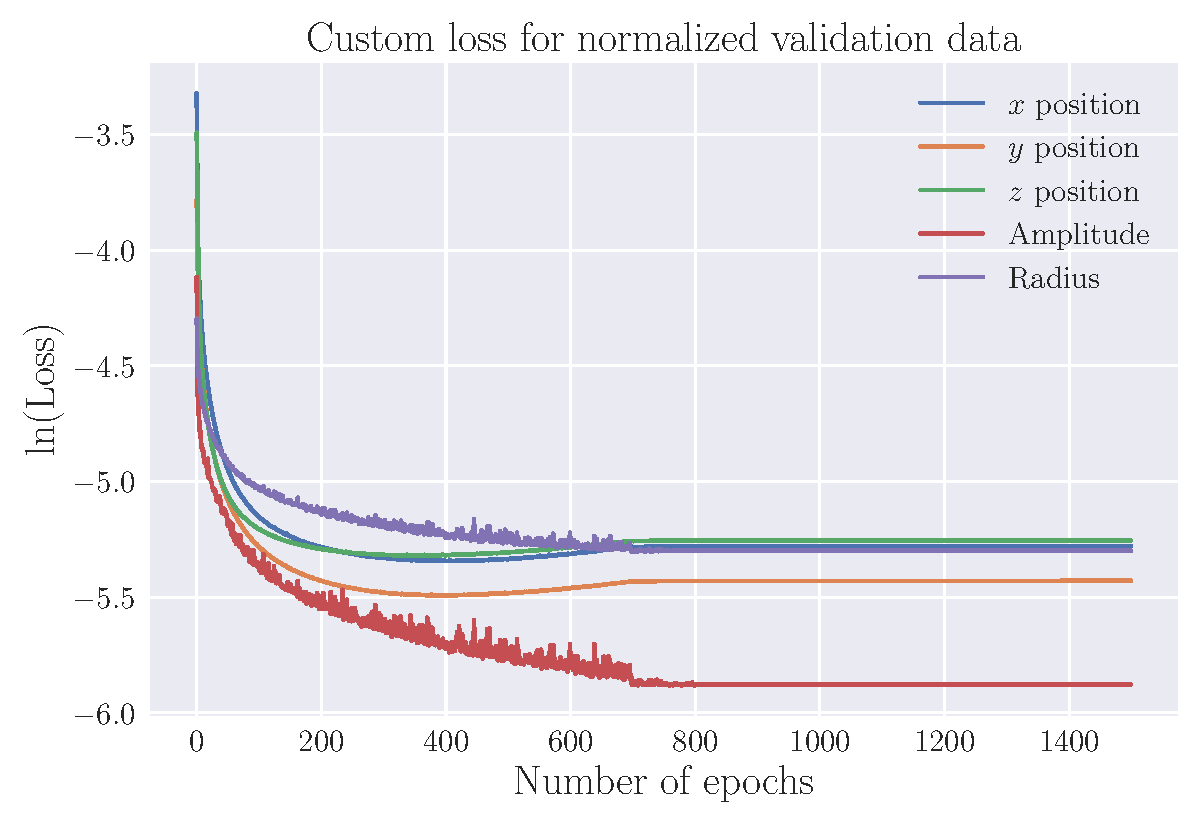
\includegraphics[width=\linewidth]{figures/NN_area/Custom_Loss_mse_targets_area_seed_42_cnn_32_0.001_0.35_0.1_0_1500_(0).pdf}
    \caption{Validation MSE loss as a function of epoch for each target value, including the $x$-, $y$-, and $z$-coordinates of the center of the dipole population, as well as the amplitude and radius.}
    \label{fig:dipole_area_target_result}
\end{figure}

\FloatBarrier


We furter evaluate our model's predictions, by feeding it with unseen test data. By denormalizing the output of the network and comparing it to the target values the MED between the predicted and target coordinates measures to 7.85 mm, MAE between predicted and target magnitude equals 0.33 nAm and MAE between predicted and target radius is 0.76 mm. The MED measures a slightly higher value compared to when predicting only position and magnitude strength of the dipole. However, we note that the MAE corresponding to the magnitude has decreased in this more complex problem, now corresponding to a relative error of only 3.67$\%$. In table \ref{tab:Loss_dipole_area} we can read off the percentages of the network predictions of test samples that falls within various threshold values. We have that 79.68 $\%$ of the predictions has a ED in position smaller than 10 mm, 98.57$\%$ an AE in magnitude smaller than 2 nAm and 97.22$\%$ an AE in radius smaller than 3 mm.

Table \ref{tab:thresholds_dipole_area} further provides an overview of the percentage of samples that fulfill multiple of threshold values at once. These numbers have been found with the initial condition that all predictions fulfill the constraint that the ED between predicted and target position is smaller than 10 mm. A result drawn from the table is that 78.290$\%$ of the FFNN's predictions have an AE smaller than 2 nAm in magnitude and 3 mm in radius.


\begin{table}[]
\hspace*{-2.8cm}
\begin{tabular}{|ccc|l|ccc|l|ccc|}
\cline{1-3} \cline{5-7} \cline{9-11}
\multicolumn{3}{|c|}{\cellcolor[HTML]{CBCEFB}\textbf{Eucledian Distance: Position}}                                                                                                                                                                                                                             & \textbf{}             & \multicolumn{3}{c|}{\cellcolor[HTML]{CBCEFB}\textbf{Absolute Error: Magnitude}}                                                                                                                                                                                                                             & \textbf{}             & \multicolumn{3}{c|}{\cellcolor[HTML]{CBCEFB}\textbf{Absolute Error: Radius}}                                                                                                                                                                                                                                   \\ \cline{1-3} \cline{5-7} \cline{9-11}
\multicolumn{1}{|c|}{\cellcolor[HTML]{EFEFEF}\begin{tabular}[c]{@{}c@{}}ED \\ \textless 5 mm\end{tabular}} & \multicolumn{1}{c|}{\cellcolor[HTML]{EFEFEF}\begin{tabular}[c]{@{}c@{}}ED \\ \textless 10 mm\end{tabular}} & \cellcolor[HTML]{EFEFEF}\begin{tabular}[c]{@{}c@{}}ED \\ \textless 15 mm\end{tabular} &                       & \multicolumn{1}{c|}{\cellcolor[HTML]{EFEFEF}\begin{tabular}[c]{@{}c@{}}AE \\ \textless 1 nAm\end{tabular}} & \multicolumn{1}{c|}{\cellcolor[HTML]{EFEFEF}\begin{tabular}[c]{@{}c@{}}AE\\ \textless 2 nAm\end{tabular}} & \cellcolor[HTML]{EFEFEF}\begin{tabular}[c]{@{}c@{}}AE \\ \textless 3 nAm\end{tabular} &                       & \multicolumn{1}{c|}{\cellcolor[HTML]{EFEFEF}\begin{tabular}[c]{@{}c@{}}AE \\ \textless 1 mm\end{tabular}} & \multicolumn{1}{c|}{\cellcolor[HTML]{EFEFEF}\begin{tabular}[c]{@{}c@{}}AE \\ \textless 3 mm\end{tabular}} & \cellcolor[HTML]{EFEFEF}\begin{tabular}[c]{@{}c@{}}AE \\ \textless 5 mm\end{tabular} \\ \cline{1-3} \cline{5-7} \cline{9-11}
\multicolumn{1}{|c|}{56.045$\%$}                                                                           & \multicolumn{1}{c|}{79.680$\%$}                                                                            & 86.435$\%$                                                                            & \multicolumn{1}{c|}{} & \multicolumn{1}{c|}{92.900$\%$}                                                                           & \multicolumn{1}{c|}{98.565$\%$}                                                                          & 99.685$\%$                                                                           & \multicolumn{1}{c|}{} & \multicolumn{1}{c|}{74.210$\%$}                                                                           & \multicolumn{1}{c|}{98.220$\%$}                                                                            & 99.770$\%$                                                                            \\ \cline{1-3} \cline{5-7} \cline{9-11}
\end{tabular}
\caption{}
\label{table:Loss_dipole_area}
\end{table}

\begin{table}[]
\begin{tabular}{l|ccc|}
\cline{2-4}
& \multicolumn{3}{c|}{\cellcolor[HTML]{CBCEFB}\textbf{\begin{tabular}[c]{@{}c@{}}Predictions within different thresholds\\ (Initial condition for position: ED \textless 10 mm)\end{tabular}}} \\ \cline{2-4}
& \multicolumn{1}{l|}{\cellcolor[HTML]{EFEFEF}AE \textless 1 nAm} & \multicolumn{1}{l|}{\cellcolor[HTML]{EFEFEF}AE \textless 2 nAm} & \multicolumn{1}{l|}{\cellcolor[HTML]{EFEFEF}AE \textless 3 nAm} \\ \hline
\multicolumn{1}{|l|}{\cellcolor[HTML]{EFEFEF}AE \textless 1 mm} & \multicolumn{1}{c|}{58.075 $\%$} & \multicolumn{1}{c|}{59.940 $\%$} & 60.055 $\%$ \\ \hline
\multicolumn{1}{|l|}{\cellcolor[HTML]{EFEFEF}AE \textless 3 mm} & \multicolumn{1}{c|}{74.045 $\%$} & \multicolumn{1}{c|}{78.290 $\%$} & 78.765 $\%$ \\ \hline
\multicolumn{1}{|l|}{\cellcolor[HTML]{EFEFEF}AE \textless 5 mm} & \multicolumn{1}{c|}{74.315 $\%$} & \multicolumn{1}{c|}{78.890 $\%$} & 79.515 $\%$ \\ \hline
\end{tabular}
\caption{\textbf{Evaluation of the Extended FFNN utilizing different Error Metrics.}
Performance of the extended FFNN on a test data set consisting of 20,000 samples. The errors are measured using Mean Absolute Error (MAE), Mean Absolute Percentage Error (MAPE), Mean Squared Error (MSE), and Root Mean Squared Error (RMSE) for various target values.}
\label{tab:thresholds_dipole_area}
\end{table}

To ensure the model's accuracy is comparable to the work done by others and to further assess its ability to predict the center of dipole populations, in addition to magnitude and radius, we employ the same evaluation metrics as in previous problems: MAE, MSE, and RMSE. The results for these error metrics are presented in Table \ref{table:error_dipole_area}.

The MAEs for the target coordinates, i.e., the center of the dipole population, average at 3.96 mm. This is the highest MAE measured among the predictions made by the network across all the problems studied. As observed when predicting both the magnitude and position in the previous problem, the $z$-coordinate contributes the most to this MAE.

Concerning the MSE, we observe relatively small errors for amplitude and radius, with values of 0.312 and 1.114 mm$^2$, respectively. The MSE between the predicted and target coordinates ranges from 42.58 mm$^2$ to 66.816 mm$^2$, indicating the widest spread of errors compared to the previous problems studied. An increase in RMSE is also evident. This suggests that, on average, the prediction errors do not always align with the overall spread of errors. In other words, the model sometimes provides accurate predictions, while in other cases, it does not. This indicates a lower level of stability and predictability in the error distribution compared to the other problems studied.



\begin{table}
\begin{tabular}{c|
>{\columncolor[HTML]{FFFFFF}}c
>{\columncolor[HTML]{FFFFFF}}c
>{\columncolor[HTML]{FFFFFF}}c
>{\columncolor[HTML]{FFFFFF}}c
>{\columncolor[HTML]{FFFFFF}}c
>{\columncolor[HTML]{FFFFFF}}c |}
\cline{2-7}
\multicolumn{1}{l|}{} & \multicolumn{6}{c|}{\cellcolor[HTML]{CBCEFB}\textbf{Error for different target values}} \\ \cline{2-7}
\multicolumn{1}{l|}{} & \multicolumn{1}{c|}{\cellcolor[HTML]{EFEFEF}\begin{tabular}[c]{@{}c@{}}x \\ {[}mm{]}\end{tabular}} & \multicolumn{1}{c|}{\cellcolor[HTML]{EFEFEF}\begin{tabular}[c]{@{}c@{}}y \\ {[}mm{]}\end{tabular}} & \multicolumn{1}{c|}{\cellcolor[HTML]{EFEFEF}\begin{tabular}[c]{@{}c@{}}z \\ {[}mm{]}\end{tabular}} & \multicolumn{1}{l|}{\cellcolor[HTML]{EFEFEF}\begin{tabular}[c]{@{}l@{}}Center \\ {[}mm{]}\end{tabular}} & \multicolumn{1}{l|}{\cellcolor[HTML]{EFEFEF}\begin{tabular}[c]{@{}l@{}}Magnitude \\ {[}nAm{]}\end{tabular}} & \multicolumn{1}{l|}{\cellcolor[HTML]{EFEFEF}\begin{tabular}[c]{@{}l@{}}Radius \\ {[}mm{]}\end{tabular}} \\ \hline
\multicolumn{1}{|c|}{\cellcolor[HTML]{EFEFEF}MAE} & \multicolumn{1}{c|}{\cellcolor[HTML]{FFFFFF}3.819} & \multicolumn{1}{c|}{\cellcolor[HTML]{FFFFFF}4.342} & \multicolumn{1}{c|}{\cellcolor[HTML]{FFFFFF}3.722} & \multicolumn{1}{c|}{\cellcolor[HTML]{FFFFFF}3.961} & \multicolumn{1}{c|}{\cellcolor[HTML]{FFFFFF}0.325} & 0.765 \\ \hline
\multicolumn{1}{|c|}{\cellcolor[HTML]{EFEFEF}MSE} & \multicolumn{1}{c|}{\cellcolor[HTML]{FFFFFF}42.581} & \multicolumn{1}{c|}{\cellcolor[HTML]{FFFFFF}66.816} & \multicolumn{1}{c|}{\cellcolor[HTML]{FFFFFF}41.681} & \multicolumn{1}{c|}{\cellcolor[HTML]{FFFFFF}50.359} & \multicolumn{1}{c|}{\cellcolor[HTML]{FFFFFF}0.313} & 1.114 \\ \hline
\multicolumn{1}{|c|}{\cellcolor[HTML]{EFEFEF}RMSE} & \multicolumn{1}{c|}{\cellcolor[HTML]{FFFFFF}6.525} & \multicolumn{1}{c|}{\cellcolor[HTML]{FFFFFF}8.174} & \multicolumn{1}{c|}{\cellcolor[HTML]{FFFFFF}6.456} & \multicolumn{1}{c|}{\cellcolor[HTML]{FFFFFF}7.096} & \multicolumn{1}{c|}{\cellcolor[HTML]{FFFFFF}0.559} & 1.056 \\ \hline
\end{tabular}
\caption{\textbf{Dipole Population: Evaluation of the Extended FFNN utilizing different Error Metrics.}
Performance of the extended FFNN on a test data set consisting of 20,000 samples. The errors are measured using Mean Absolute Error, Mean Squared Error, and Root Mean Squared Error for various target values.}
\label{table:error_dipole_area}
\end{table}

In Figure \ref{fig:area_errors}, we present the MAE and MSE metrics calculated between the predicted and target population center values as functions of radius. The panels within the figure do not indicate any significant correlation between the size of a dipole population and the predictive error regarding its center. This observation aligns with the correlation coefficients, which are approximately 0.01 for AE and 0.00 for SE in the prediction of the center.

The panels also reveal that the majority of the samples are predicted with an absolute error smaller than 15 mm. Moreover, the left panel illustrates that the network predictions on the test samples result in a mean error larger than 1000 mm$^2$. This suggests a comparatively lower level of stability and predictability in the error distribution, in contrast to the other problems studied.


\begin{figure}
  \hspace*{-2.5cm} % Adjust the value as needed to move the figures left
  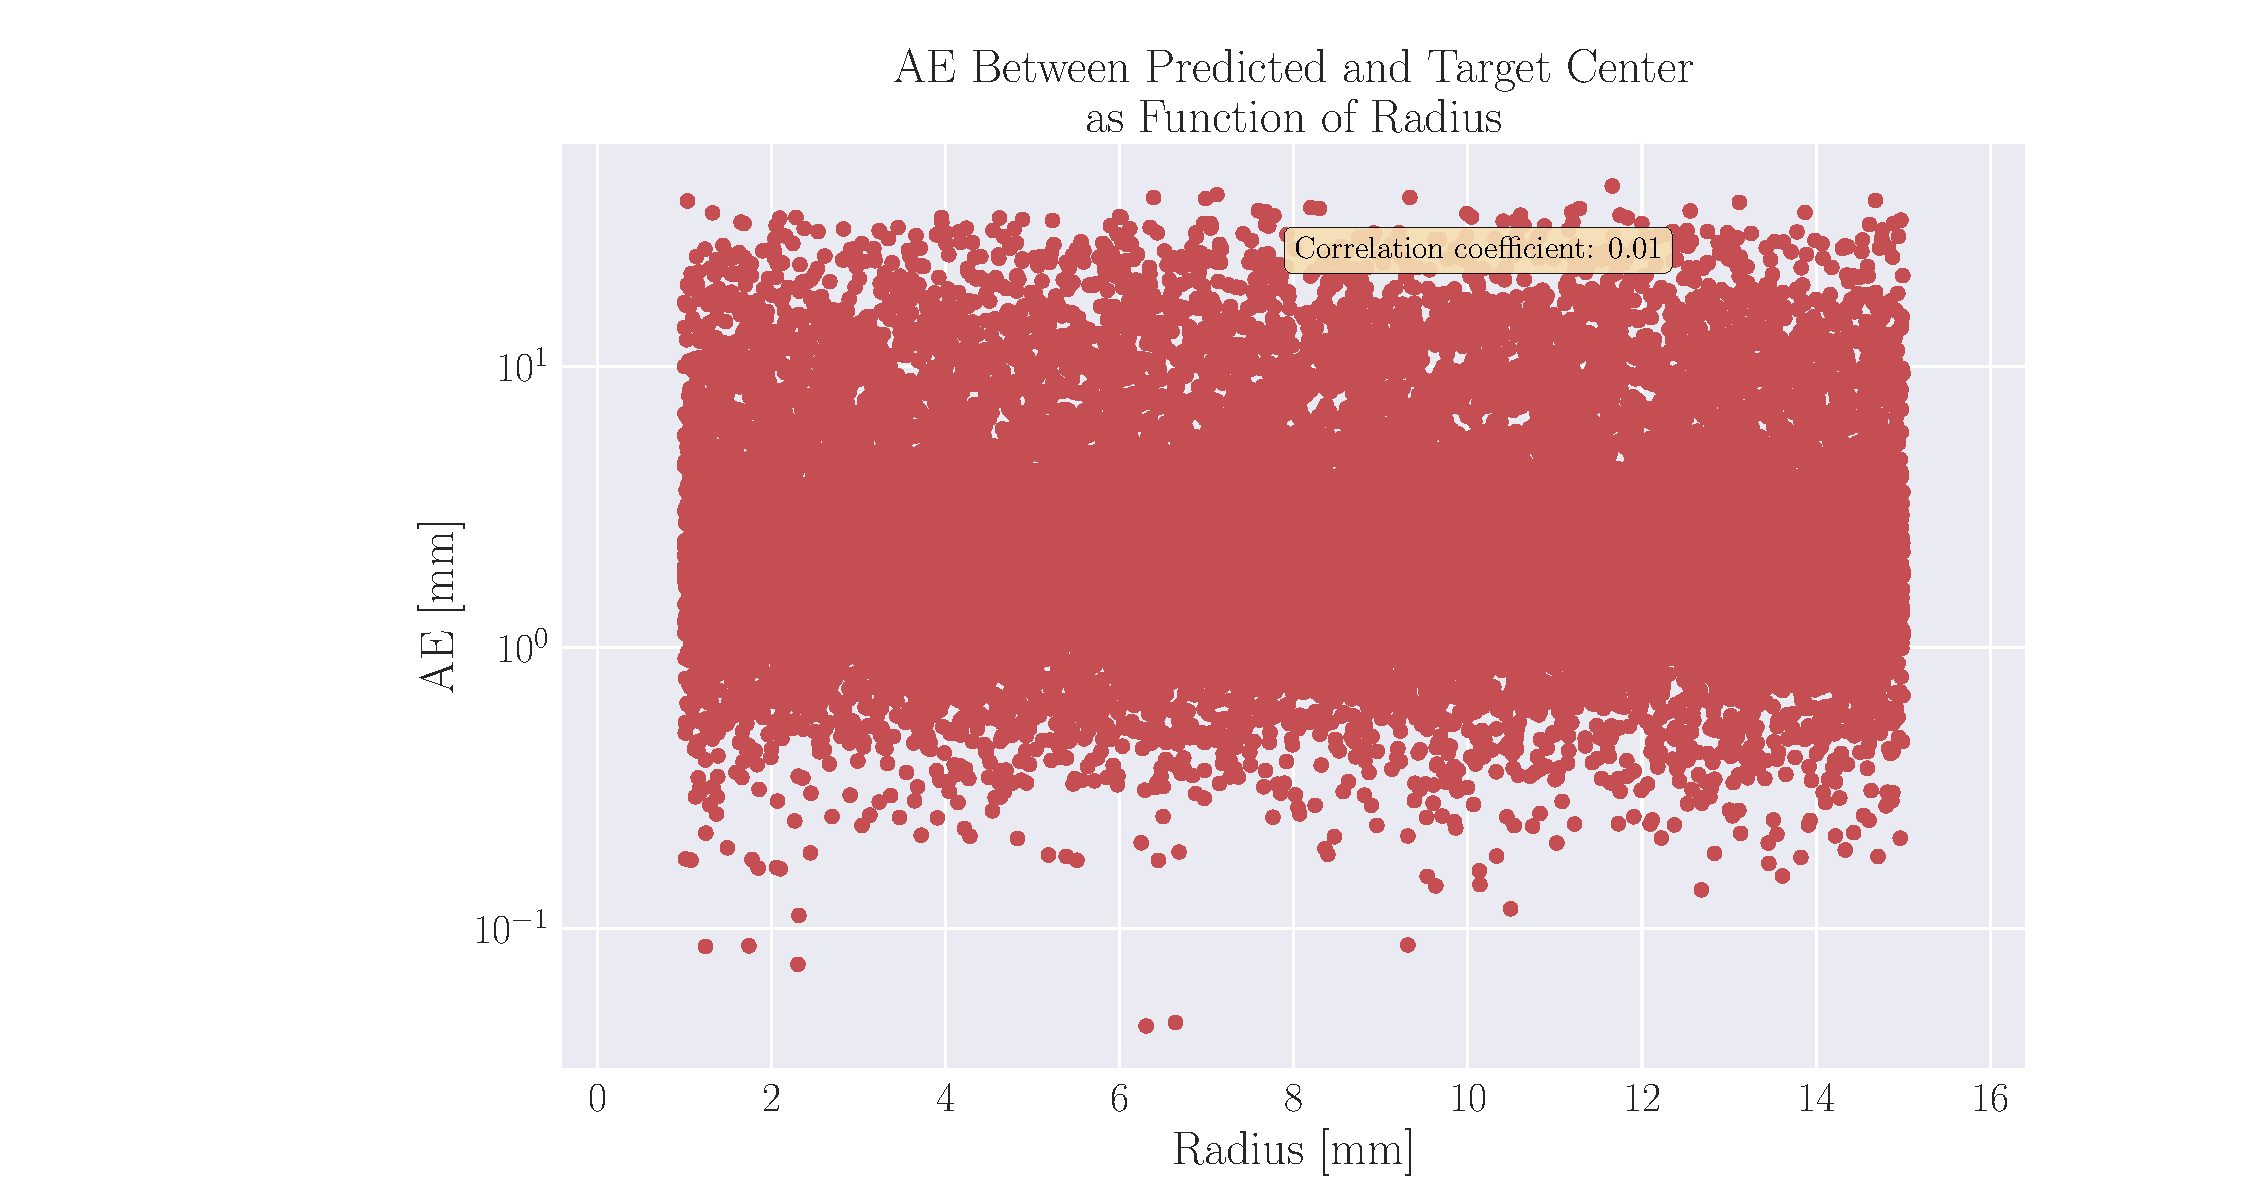
\includegraphics[width=9cm]{figures/mae_area.pdf}
  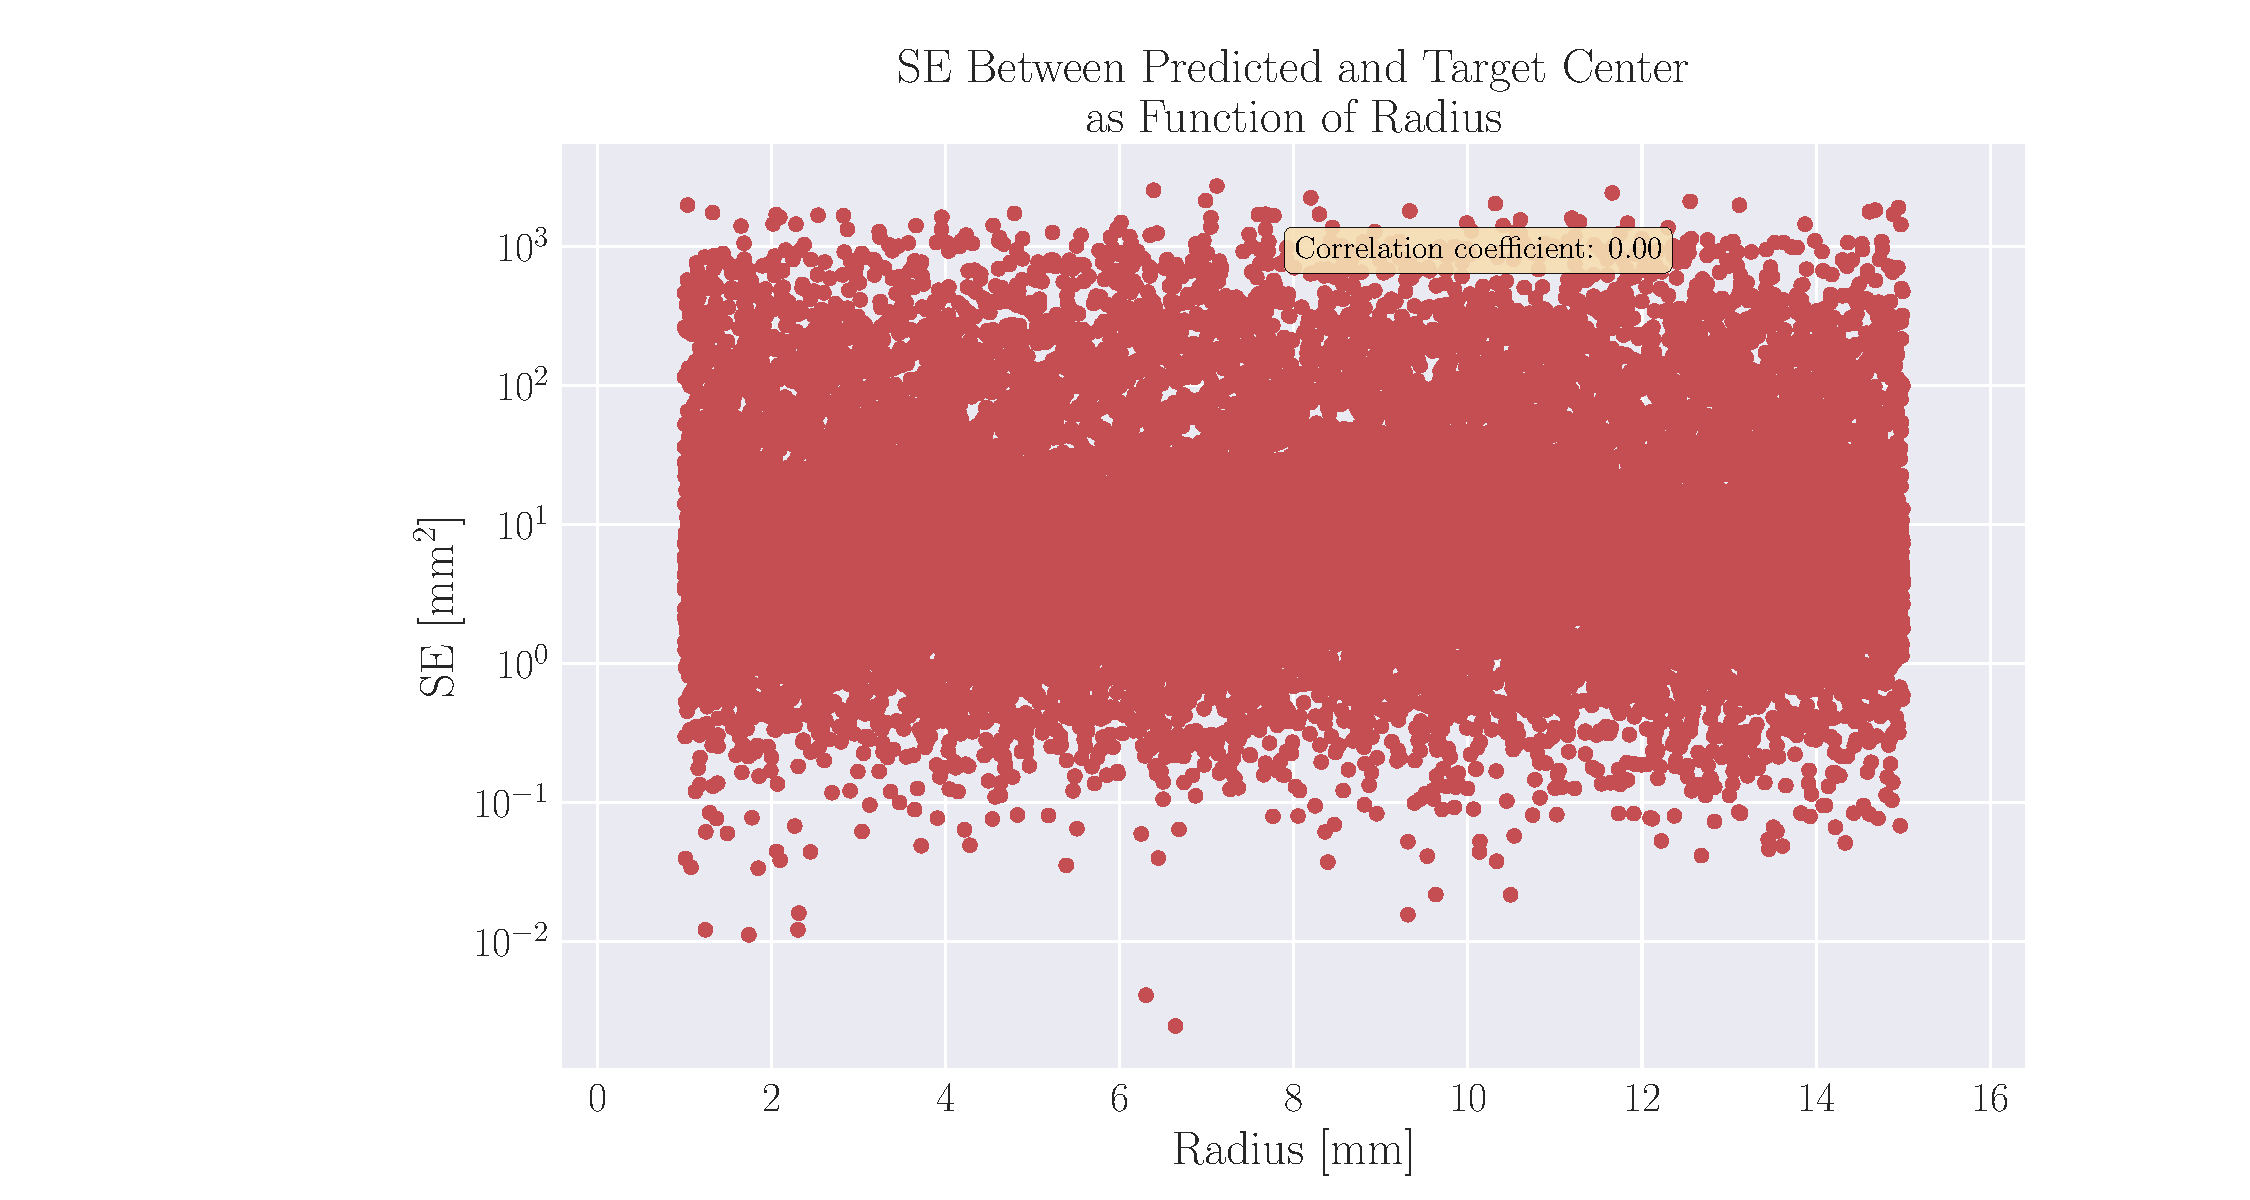
\includegraphics[width=9cm]{figures/mse_area.pdf}
  \caption{\textbf{Dipole Population:}
  Scatter plot of Mean Abolsute Error and Mean Squared Error computed between predicted and target center values, as function of the radius of the dipole populations.}
  \label{fig:area_errors}
\end{figure}


\end{document}
